% Options for packages loaded elsewhere
\PassOptionsToPackage{unicode,linktoc=all}{hyperref}
\PassOptionsToPackage{hyphens}{url}
\PassOptionsToPackage{dvipsnames,svgnames,x11names}{xcolor}
%
\documentclass[
  letterpaper,
  DIV=11,
  numbers=noendperiod]{scrreprt}

\usepackage{amsmath,amssymb}
\usepackage{lmodern}
\usepackage{iftex}
\ifPDFTeX
  \usepackage[T1]{fontenc}
  \usepackage[utf8]{inputenc}
  \usepackage{textcomp} % provide euro and other symbols
\else % if luatex or xetex
  \usepackage{unicode-math}
  \defaultfontfeatures{Scale=MatchLowercase}
  \defaultfontfeatures[\rmfamily]{Ligatures=TeX,Scale=1}
\fi
% Use upquote if available, for straight quotes in verbatim environments
\IfFileExists{upquote.sty}{\usepackage{upquote}}{}
\IfFileExists{microtype.sty}{% use microtype if available
  \usepackage[]{microtype}
  \UseMicrotypeSet[protrusion]{basicmath} % disable protrusion for tt fonts
}{}
\makeatletter
\@ifundefined{KOMAClassName}{% if non-KOMA class
  \IfFileExists{parskip.sty}{%
    \usepackage{parskip}
  }{% else
    \setlength{\parindent}{0pt}
    \setlength{\parskip}{6pt plus 2pt minus 1pt}}
}{% if KOMA class
  \KOMAoptions{parskip=half}}
\makeatother
\usepackage{xcolor}
\usepackage[margin=1in,heightrounded]{geometry}
\setlength{\emergencystretch}{3em} % prevent overfull lines
\setcounter{secnumdepth}{5}
% Make \paragraph and \subparagraph free-standing
\ifx\paragraph\undefined\else
  \let\oldparagraph\paragraph
  \renewcommand{\paragraph}[1]{\oldparagraph{#1}\mbox{}}
\fi
\ifx\subparagraph\undefined\else
  \let\oldsubparagraph\subparagraph
  \renewcommand{\subparagraph}[1]{\oldsubparagraph{#1}\mbox{}}
\fi

\usepackage{color}
\usepackage{fancyvrb}
\newcommand{\VerbBar}{|}
\newcommand{\VERB}{\Verb[commandchars=\\\{\}]}
\DefineVerbatimEnvironment{Highlighting}{Verbatim}{commandchars=\\\{\}}
% Add ',fontsize=\small' for more characters per line
\usepackage{framed}
\definecolor{shadecolor}{RGB}{241,243,245}
\newenvironment{Shaded}{\begin{snugshade}}{\end{snugshade}}
\newcommand{\AlertTok}[1]{\textcolor[rgb]{0.68,0.00,0.00}{#1}}
\newcommand{\AnnotationTok}[1]{\textcolor[rgb]{0.37,0.37,0.37}{#1}}
\newcommand{\AttributeTok}[1]{\textcolor[rgb]{0.40,0.45,0.13}{#1}}
\newcommand{\BaseNTok}[1]{\textcolor[rgb]{0.68,0.00,0.00}{#1}}
\newcommand{\BuiltInTok}[1]{\textcolor[rgb]{0.00,0.23,0.31}{#1}}
\newcommand{\CharTok}[1]{\textcolor[rgb]{0.13,0.47,0.30}{#1}}
\newcommand{\CommentTok}[1]{\textcolor[rgb]{0.37,0.37,0.37}{#1}}
\newcommand{\CommentVarTok}[1]{\textcolor[rgb]{0.37,0.37,0.37}{\textit{#1}}}
\newcommand{\ConstantTok}[1]{\textcolor[rgb]{0.56,0.35,0.01}{#1}}
\newcommand{\ControlFlowTok}[1]{\textcolor[rgb]{0.00,0.23,0.31}{#1}}
\newcommand{\DataTypeTok}[1]{\textcolor[rgb]{0.68,0.00,0.00}{#1}}
\newcommand{\DecValTok}[1]{\textcolor[rgb]{0.68,0.00,0.00}{#1}}
\newcommand{\DocumentationTok}[1]{\textcolor[rgb]{0.37,0.37,0.37}{\textit{#1}}}
\newcommand{\ErrorTok}[1]{\textcolor[rgb]{0.68,0.00,0.00}{#1}}
\newcommand{\ExtensionTok}[1]{\textcolor[rgb]{0.00,0.23,0.31}{#1}}
\newcommand{\FloatTok}[1]{\textcolor[rgb]{0.68,0.00,0.00}{#1}}
\newcommand{\FunctionTok}[1]{\textcolor[rgb]{0.28,0.35,0.67}{#1}}
\newcommand{\ImportTok}[1]{\textcolor[rgb]{0.00,0.46,0.62}{#1}}
\newcommand{\InformationTok}[1]{\textcolor[rgb]{0.37,0.37,0.37}{#1}}
\newcommand{\KeywordTok}[1]{\textcolor[rgb]{0.00,0.23,0.31}{#1}}
\newcommand{\NormalTok}[1]{\textcolor[rgb]{0.00,0.23,0.31}{#1}}
\newcommand{\OperatorTok}[1]{\textcolor[rgb]{0.37,0.37,0.37}{#1}}
\newcommand{\OtherTok}[1]{\textcolor[rgb]{0.00,0.23,0.31}{#1}}
\newcommand{\PreprocessorTok}[1]{\textcolor[rgb]{0.68,0.00,0.00}{#1}}
\newcommand{\RegionMarkerTok}[1]{\textcolor[rgb]{0.00,0.23,0.31}{#1}}
\newcommand{\SpecialCharTok}[1]{\textcolor[rgb]{0.37,0.37,0.37}{#1}}
\newcommand{\SpecialStringTok}[1]{\textcolor[rgb]{0.13,0.47,0.30}{#1}}
\newcommand{\StringTok}[1]{\textcolor[rgb]{0.13,0.47,0.30}{#1}}
\newcommand{\VariableTok}[1]{\textcolor[rgb]{0.07,0.07,0.07}{#1}}
\newcommand{\VerbatimStringTok}[1]{\textcolor[rgb]{0.13,0.47,0.30}{#1}}
\newcommand{\WarningTok}[1]{\textcolor[rgb]{0.37,0.37,0.37}{\textit{#1}}}

\providecommand{\tightlist}{%
  \setlength{\itemsep}{0pt}\setlength{\parskip}{0pt}}\usepackage{longtable,booktabs,array}
\usepackage{calc} % for calculating minipage widths
% Correct order of tables after \paragraph or \subparagraph
\usepackage{etoolbox}
\makeatletter
\patchcmd\longtable{\par}{\if@noskipsec\mbox{}\fi\par}{}{}
\makeatother
% Allow footnotes in longtable head/foot
\IfFileExists{footnotehyper.sty}{\usepackage{footnotehyper}}{\usepackage{footnote}}
\makesavenoteenv{longtable}
\usepackage{graphicx}
\makeatletter
\def\maxwidth{\ifdim\Gin@nat@width>\linewidth\linewidth\else\Gin@nat@width\fi}
\def\maxheight{\ifdim\Gin@nat@height>\textheight\textheight\else\Gin@nat@height\fi}
\makeatother
% Scale images if necessary, so that they will not overflow the page
% margins by default, and it is still possible to overwrite the defaults
% using explicit options in \includegraphics[width, height, ...]{}
\setkeys{Gin}{width=\maxwidth,height=\maxheight,keepaspectratio}
% Set default figure placement to htbp
\makeatletter
\def\fps@figure{htbp}
\makeatother
\newlength{\cslhangindent}
\setlength{\cslhangindent}{1.5em}
\newlength{\csllabelwidth}
\setlength{\csllabelwidth}{3em}
\newlength{\cslentryspacingunit} % times entry-spacing
\setlength{\cslentryspacingunit}{\parskip}
\newenvironment{CSLReferences}[2] % #1 hanging-ident, #2 entry spacing
 {% don't indent paragraphs
  \setlength{\parindent}{0pt}
  % turn on hanging indent if param 1 is 1
  \ifodd #1
  \let\oldpar\par
  \def\par{\hangindent=\cslhangindent\oldpar}
  \fi
  % set entry spacing
  \setlength{\parskip}{#2\cslentryspacingunit}
 }%
 {}
\usepackage{calc}
\newcommand{\CSLBlock}[1]{#1\hfill\break}
\newcommand{\CSLLeftMargin}[1]{\parbox[t]{\csllabelwidth}{#1}}
\newcommand{\CSLRightInline}[1]{\parbox[t]{\linewidth - \csllabelwidth}{#1}\break}
\newcommand{\CSLIndent}[1]{\hspace{\cslhangindent}#1}

\usepackage{makeidx}
\makeindex
\KOMAoption{captions}{tableheading}
\makeatletter
\makeatother
\makeatletter
\@ifpackageloaded{bookmark}{}{\usepackage{bookmark}}
\makeatother
\makeatletter
\@ifpackageloaded{caption}{}{\usepackage{caption}}
\AtBeginDocument{%
\ifdefined\contentsname
  \renewcommand*\contentsname{Table of contents}
\else
  \newcommand\contentsname{Table of contents}
\fi
\ifdefined\listfigurename
  \renewcommand*\listfigurename{List of Figures}
\else
  \newcommand\listfigurename{List of Figures}
\fi
\ifdefined\listtablename
  \renewcommand*\listtablename{List of Tables}
\else
  \newcommand\listtablename{List of Tables}
\fi
\ifdefined\figurename
  \renewcommand*\figurename{Figure}
\else
  \newcommand\figurename{Figure}
\fi
\ifdefined\tablename
  \renewcommand*\tablename{Table}
\else
  \newcommand\tablename{Table}
\fi
}
\@ifpackageloaded{float}{}{\usepackage{float}}
\floatstyle{ruled}
\@ifundefined{c@chapter}{\newfloat{codelisting}{h}{lop}}{\newfloat{codelisting}{h}{lop}[chapter]}
\floatname{codelisting}{Listing}
\newcommand*\listoflistings{\listof{codelisting}{List of Listings}}
\makeatother
\makeatletter
\@ifpackageloaded{caption}{}{\usepackage{caption}}
\@ifpackageloaded{subcaption}{}{\usepackage{subcaption}}
\makeatother
\makeatletter
\@ifpackageloaded{tcolorbox}{}{\usepackage[many]{tcolorbox}}
\makeatother
\makeatletter
\@ifundefined{shadecolor}{\definecolor{shadecolor}{rgb}{.97, .97, .97}}
\makeatother
\makeatletter
\makeatother
\ifLuaTeX
  \usepackage{selnolig}  % disable illegal ligatures
\fi
\IfFileExists{bookmark.sty}{\usepackage{bookmark}}{\usepackage{hyperref}}
\IfFileExists{xurl.sty}{\usepackage{xurl}}{} % add URL line breaks if available
\urlstyle{same} % disable monospaced font for URLs
\hypersetup{
  pdftitle={Business Statistics},
  pdfauthor={J. Alejandro Gelves},
  colorlinks=true,
  linkcolor={blue},
  filecolor={Maroon},
  citecolor={Blue},
  urlcolor={Blue},
  pdfcreator={LaTeX via pandoc}}

\title{Business Statistics}
\usepackage{etoolbox}
\makeatletter
\providecommand{\subtitle}[1]{% add subtitle to \maketitle
  \apptocmd{\@title}{\par {\large #1 \par}}{}{}
}
\makeatother
\subtitle{A Guide for BUAD 231}
\author{J. Alejandro Gelves}
\date{12/27/22}

\begin{document}
\maketitle
\ifdefined\Shaded\renewenvironment{Shaded}{\begin{tcolorbox}[boxrule=0pt, enhanced, breakable, colback={shadecolor}, frame hidden]}{\end{tcolorbox}}\fi

\renewcommand*\contentsname{Table of contents}
{
\hypersetup{linkcolor=}
\setcounter{tocdepth}{1}
\tableofcontents
}
\bookmarksetup{startatroot}

\hypertarget{introduction}{%
\chapter*{Introduction}\label{introduction}}
\addcontentsline{toc}{chapter}{Introduction}

\markboth{Introduction}{Introduction}

``Whatever you would make habitual, practice it; and if you would not
make a thing habitual, do not practice it, but accustom yourself to
something else.'' \emph{Epictetus}

How often do we feel bad about ourselves because we procrastinated,
squandered our time, or did not accomplish something meaningful during
the day? Making the right decisions takes practice. In this book, I
invite you to practice the skills you have learned in BUAD 231 and the
skills of focus, dedication, and consistency. Choose a day in the week
and start by dedicating some fixed time to these problems (e.g., 15-30
minutes). The idea is to work on consistency (i.e., returning to the
book weekly for a given amount of time). Some of us will find that
concentrating is challenging. Your next task is to reduce distractions
(i.e., the phone, t.v. or even your thoughts about the future). If you
keep trying and returning to the book, you will improve at Business
Statistics and learn to study with focus and consistency. All it takes
is practice. Remember, you are what you practice!

The problems in this book are designed to help you master statistics and
its application in R. I recommend reviewing Grolemund (2014) if you need
additional help learning R. Finally, I have provided a list of concepts
at the beginning of every chapter. Enjoy!

\hypertarget{why-r}{%
\section*{Why R?}\label{why-r}}
\addcontentsline{toc}{section}{Why R?}

\markright{Why R?}

We will be using R to apply the lessons we learn in BUAD 231. R is a
language and environment for statistical computing and graphics. There
are several advantages to using the R software for statistical analysis
and data science. Some of the main benefits include:

\begin{itemize}
\item
  R is a \textbf{powerful and flexible programming language} that allows
  users to manipulate and analyze data in many different ways.
\item
  R has a large and \textbf{active community of users}, who have
  developed a wide range of packages and tools for data analysis and
  visualization.
\item
  R is \textbf{free and open-source}, which makes it accessible to
  anyone who wants to use it.
\item
  R is \textbf{widely used} in academia and industry, which means that
  there are many resources and tutorials available to help users learn
  how to use it.
\item
  R is well-suited for working with \textbf{large and complex datasets},
  and it can handle data from many different sources.
\item
  R can be \textbf{easily integrated} with other tools and software,
  such as databases, visualization tools, and machine learning
  algorithms.
\end{itemize}

Overall, R is a powerful and versatile tool for data analysis and data
science, and it offers many benefits to users who want to work with
data.

\hypertarget{installing-r}{%
\section*{Installing R}\label{installing-r}}
\addcontentsline{toc}{section}{Installing R}

\markright{Installing R}

To install R, visit the R webpage at \url{https://www.r-project.org/}.
Once in the website, click on the CRAN hyperlink.

\begin{figure}

{\centering 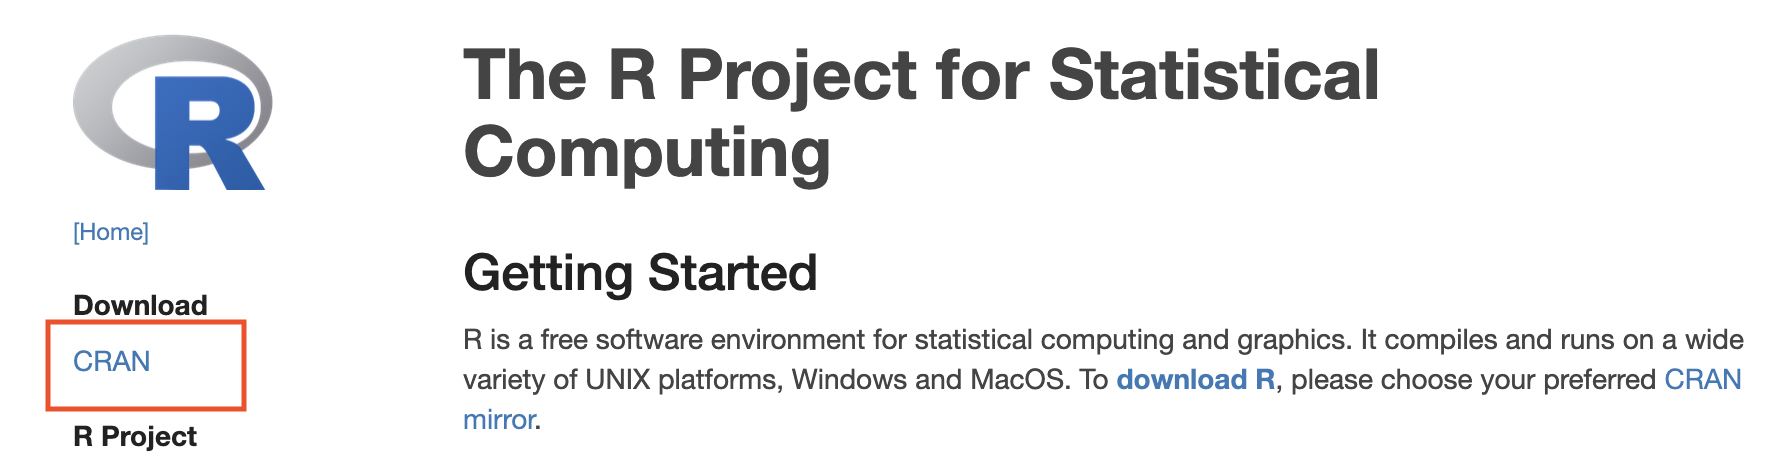
\includegraphics[width=0.75\textwidth,height=\textheight]{./images/CRAN.jpeg}

}

\end{figure}

Here you can select the CRAN mirror. Scroll down until you see USA. You
are free to choose any mirror you like, I recommend using the Duke
University mirror.

\begin{figure}

{\centering 
\includegraphics[width=0.75\textwidth,height=\textheight]{./images/DukeCRAN.jpeg}

}

\end{figure}

Once you click on the hyperlink, you will be prompted to choose the
download for your operating system. Depending on your operating system,
choose either a Windows or Macintosh download.

\begin{figure}

{\centering 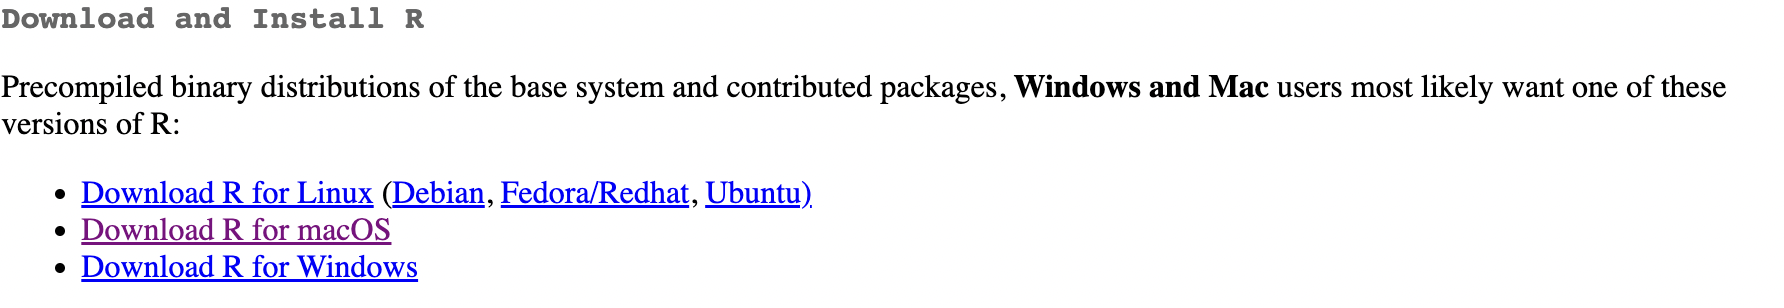
\includegraphics[width=0.75\textwidth,height=\textheight]{./images/OSDownload.jpeg}

}

\end{figure}

Follow all prompts and complete installation.

\hypertarget{installing-rstudio}{%
\section*{Installing RStudio}\label{installing-rstudio}}
\addcontentsline{toc}{section}{Installing RStudio}

\markright{Installing RStudio}

Visit the Posit website at \url{https://posit.co}. Once on the website,
hover to the top right of the screen. You will see a ``Download
RStudio'' blue button.

\begin{figure}

{\centering 
\includegraphics[width=0.75\textwidth,height=\textheight]{./images/RStudio1.jpeg}

}

\end{figure}

Next, scroll down until you reach the RStudio desktop section. Click
once more on ``Download RStudio''. You can now just jump to Step 2 since
you have already downloaded R. Finally, choose the desired download
depending on your operating system.

\begin{figure}

{\centering 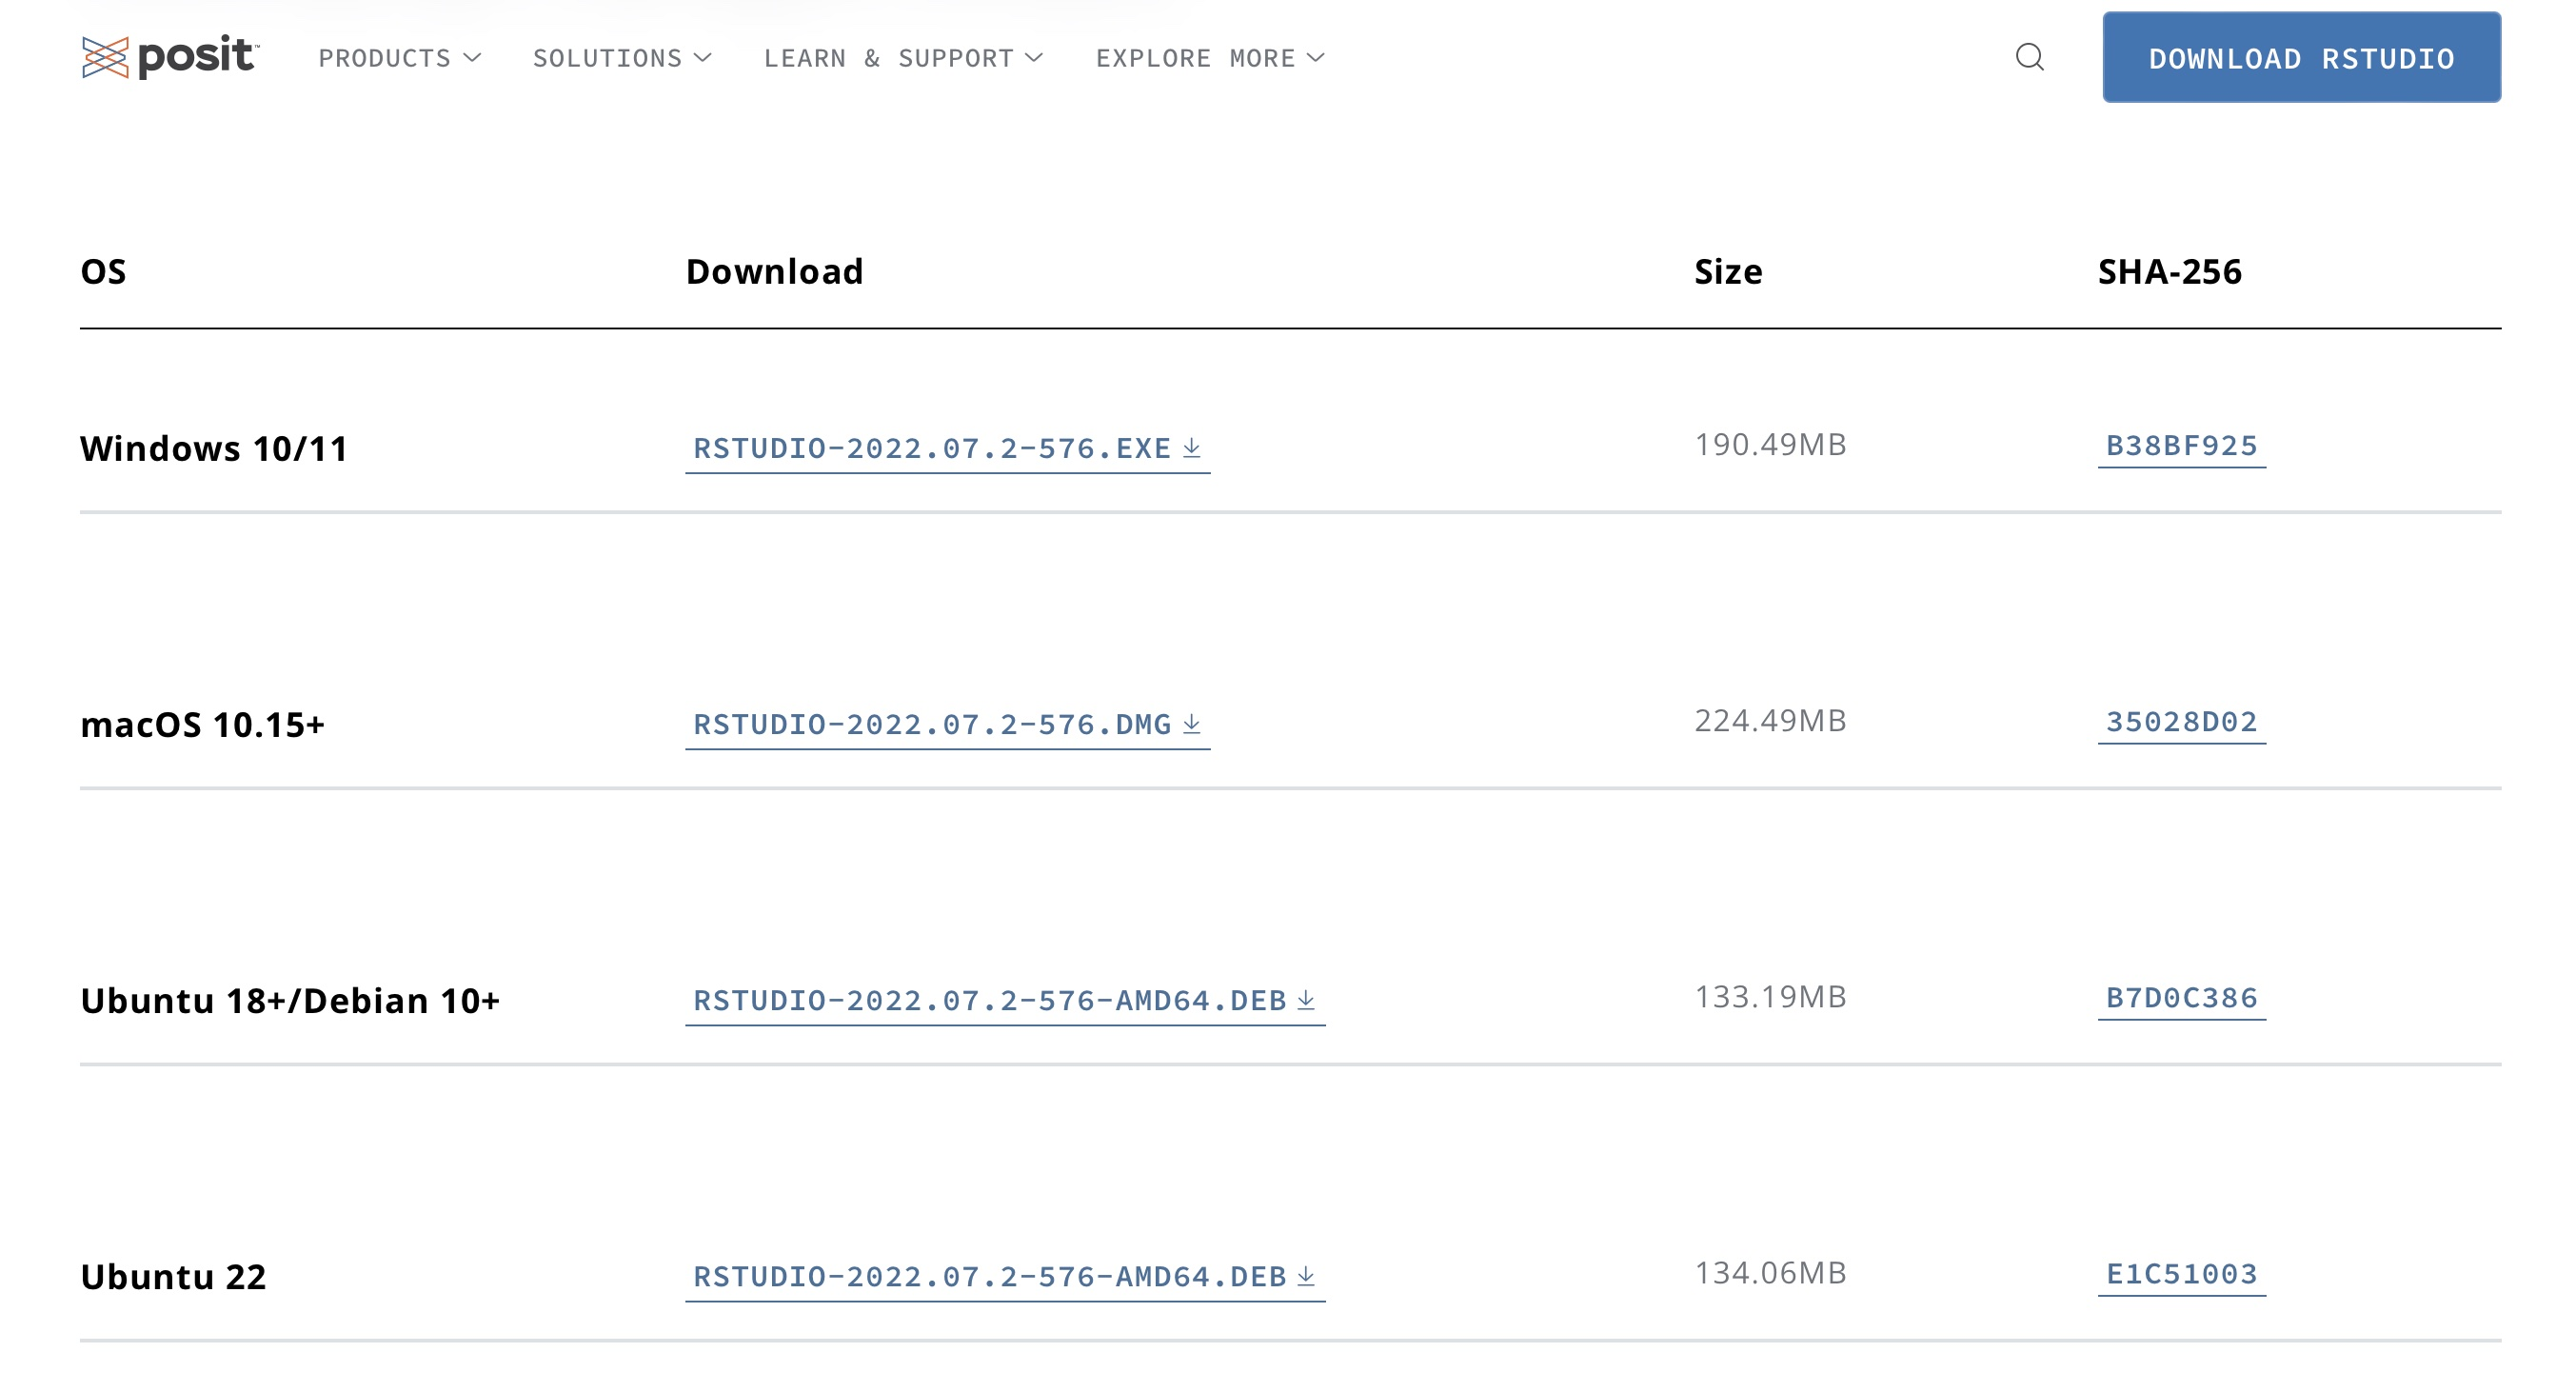
\includegraphics[width=0.75\textwidth,height=\textheight]{./images/Desktop.jpeg}

}

\end{figure}

It is important to note that RStudio will not work if R is not
installed. You can think of R as the engine and RStudio as the
interface.

\hypertarget{posit-cloud}{%
\section*{Posit Cloud}\label{posit-cloud}}
\addcontentsline{toc}{section}{Posit Cloud}

\markright{Posit Cloud}

If you do not wish to install R, you can always use the cloud version.
To do this, visit \url{https://posit.cloud/}. On the main page click on
the ``Sign Up'' button.

\begin{figure}

{\centering 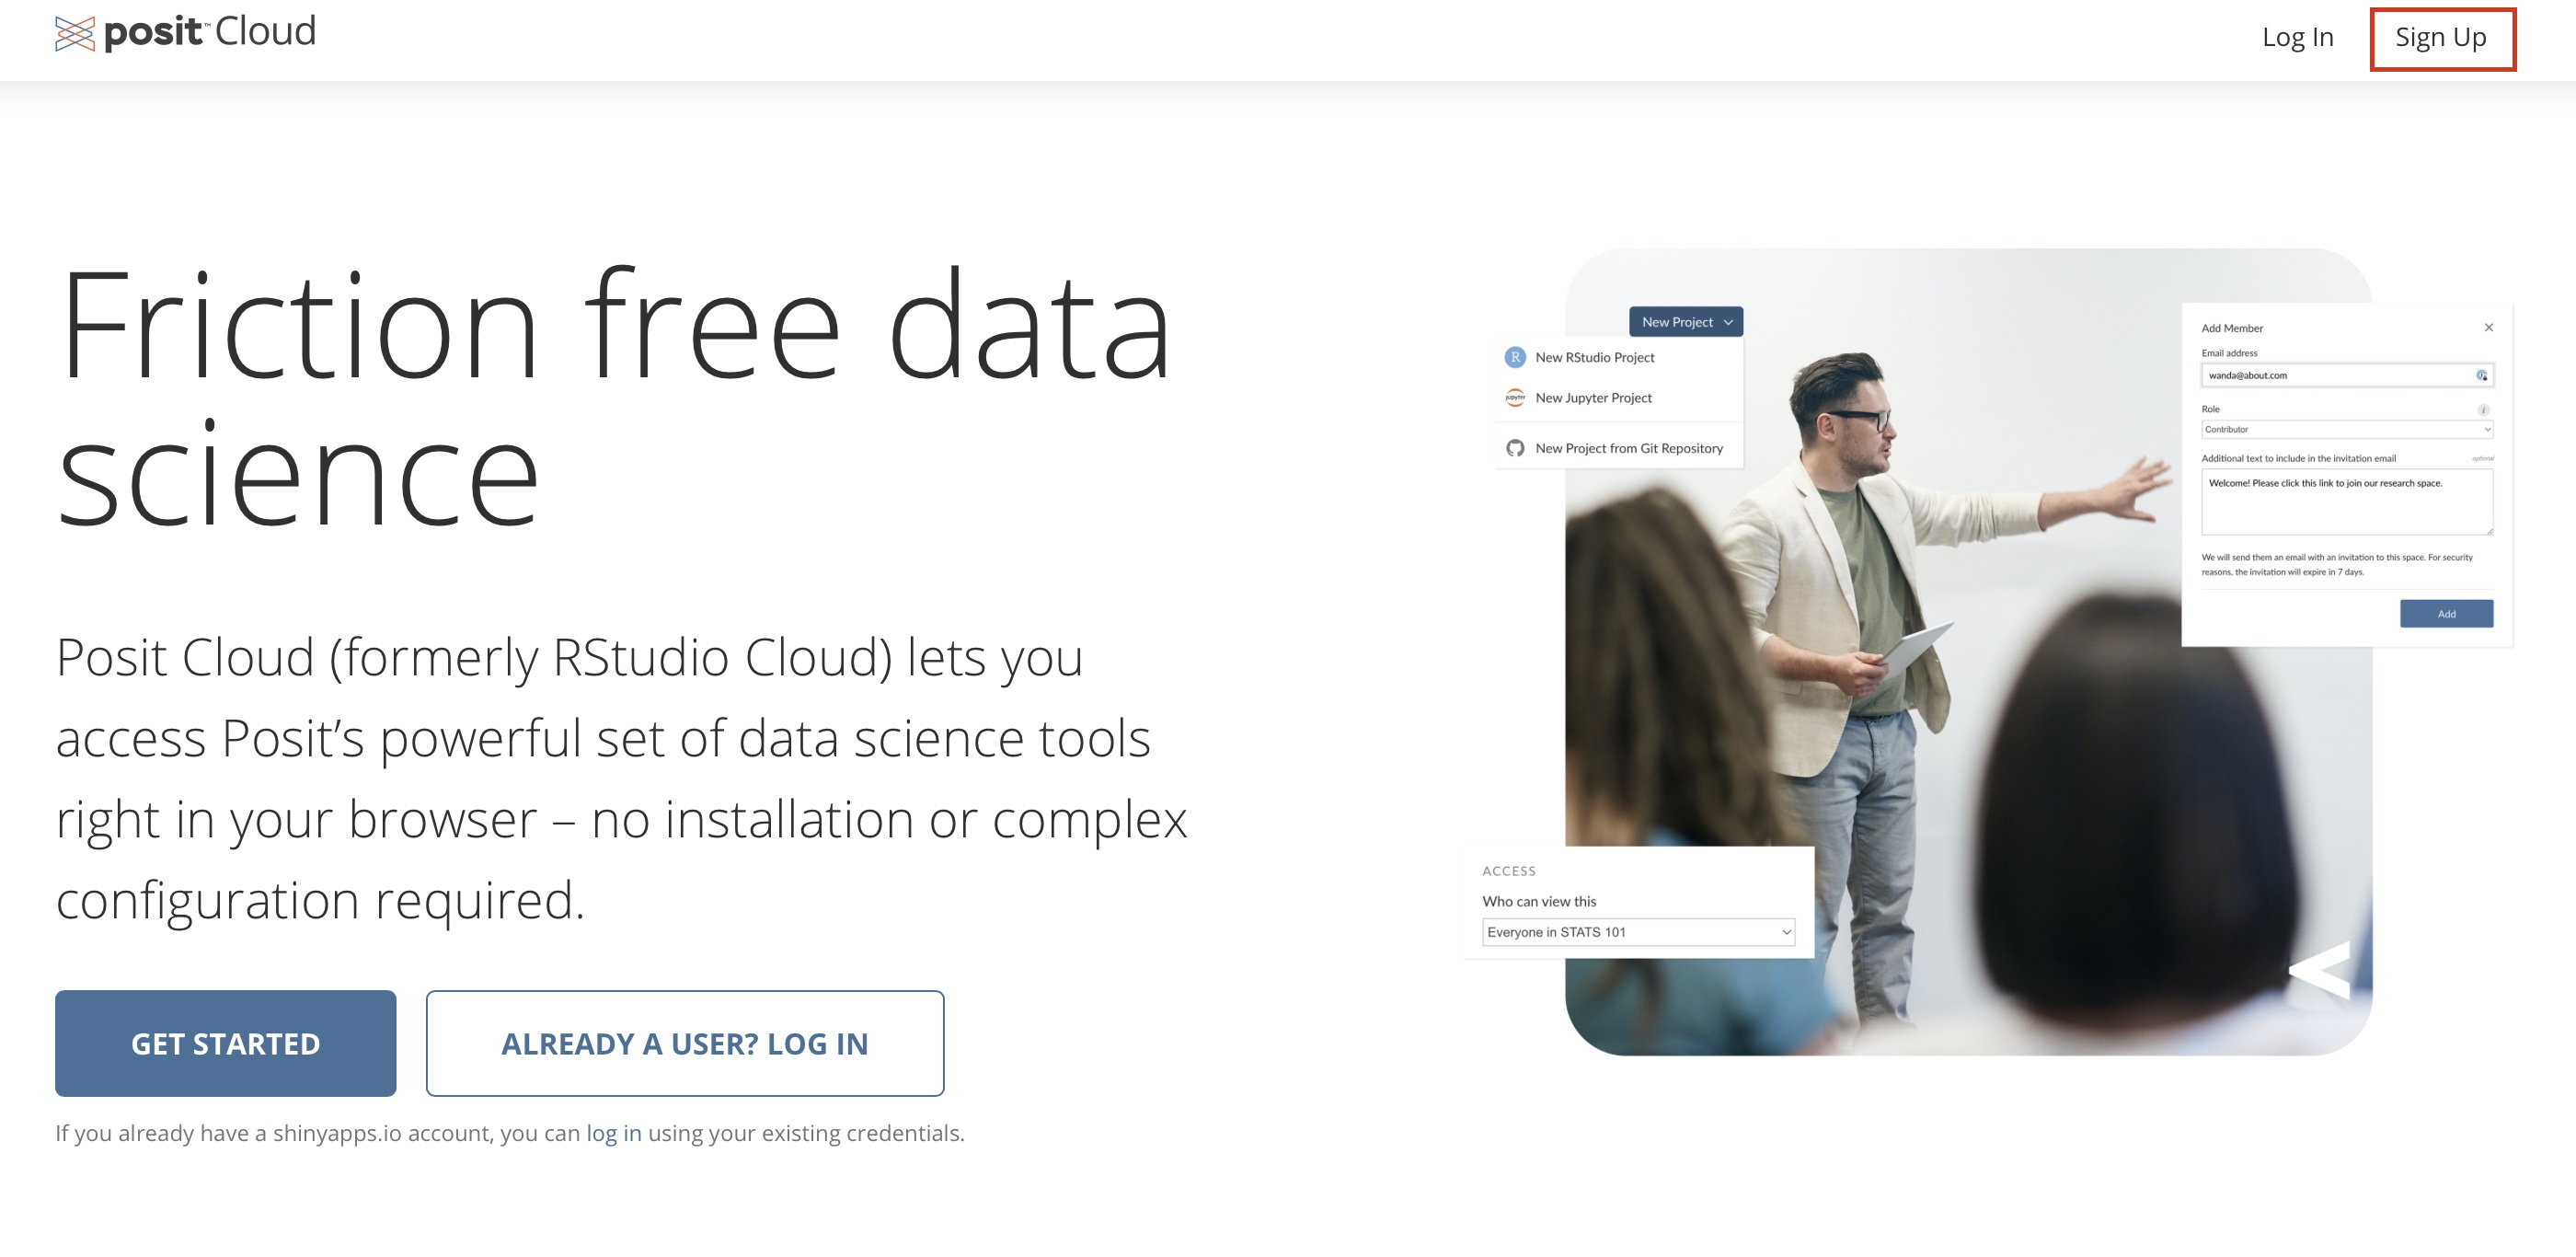
\includegraphics[width=0.75\textwidth,height=\textheight]{./images/Cloud.jpeg}

}

\end{figure}

Choose the ``Cloud Free'' option and log in using your Google
credentials (if you have a Google account) or sign up if you want to
create a new account.

\part{Descriptive Statistics}

\hypertarget{descriptive-stats-i}{%
\chapter{Descriptive Stats I}\label{descriptive-stats-i}}

\hypertarget{concepts}{%
\section{Concepts}\label{concepts}}

\hypertarget{data-and-types-of-data}{%
\subsection*{Data and Types of Data}\label{data-and-types-of-data}}
\addcontentsline{toc}{subsection}{Data and Types of Data}

\textbf{Data} are facts and figures collected, analyzed and summarized
for presentation and interpretation. Data can be classified as:

\begin{itemize}
\item
  \textbf{Cross Sectional Data} refers to data collected at the same (or
  approximately the same) point in time. Ex: NFL standings in 1980 or
  Country GDP in 2015.
\item
  \textbf{Time Series Data} refers to data collected over several time
  periods. Ex: U.S. inflation rate from 2000-2010 or Tesla deliveries
  from 2016-2022.
\item
  \textbf{Structured Data} resides in a predefined row-column format
  (tidy).
\item
  \textbf{Unstructured Data} do not conform to a pre-defined row-column
  format. Ex: Text, video, and other multimedia.
\end{itemize}

\hypertarget{data-sets-variables-and-scales-of-measurement}{%
\subsection*{Data Sets, Variables and Scales of
Measurement}\label{data-sets-variables-and-scales-of-measurement}}
\addcontentsline{toc}{subsection}{Data Sets, Variables and Scales of
Measurement}

A \textbf{data set} contains all data collected for a particular study.
Data sets are composed of:

\begin{itemize}
\item
  \textbf{Elements} are the entities on which data are collected. Ex:
  Football teams, countries, and individuals.
\item
  \textbf{Observations} are the set of measurements obtained for a
  particular element.
\item
  \textbf{Variables} are a set of characteristics collected for each
  element.
\end{itemize}

The \textbf{scales of measurements} determine the amount and type of
information contained in each variable. In general, variables can be
classified as \textbf{categorical} or \textbf{numerical}.

\begin{itemize}
\item
  \textbf{Categorical} (qualitative) data includes labels or names to
  identify an attribute of each element. Categorical data can be
  \textbf{nominal} or \textbf{ordinal}.

  \begin{itemize}
  \item
    With \textbf{nominal} data, the order of the categories is
    arbitrary. Ex: Marital Status, Race/Ethnicity, or NFL division.
  \item
    With \textbf{ordinal} data, the order or rank of the categories is
    meaningful. Ex: Rating, Difficulty Level, or Spice Level.
  \end{itemize}
\item
  \textbf{Numerical} (quantitative) include numerical values that
  indicate how many (discrete) or how much (continuous). The data can be
  either \textbf{interval} or \textbf{ratio}.

  \begin{itemize}
  \item
    With \textbf{interval} data, the distance between values is
    expressed in terms of a fixed unit of measure. The zero value is
    arbitrary and does not represent the absence of the characteristic.
    Ratios are not meaningful. Ex: Temperature or Dates.
  \item
    With \textbf{ratio} data, the ratio between values is meaningful.
    The zero value is not arbitrary and represents the absence of the
    characteristic. Ex: Prices, Profits, Wins.
  \end{itemize}
\end{itemize}

\hypertarget{useful-r-functions}{%
\subsection*{Useful R Functions}\label{useful-r-functions}}
\addcontentsline{toc}{subsection}{Useful R Functions}

Base R has some important functions that are helpful when dealing with
data. Below is a list that might come handy.

\begin{itemize}
\tightlist
\item
  The \texttt{na.omit()} function removes any observations that have a
  missing value (NA). The resulting data frame has only complete cases.
\item
  The \texttt{nrow()} and \texttt{ncol()} functions return the number of
  rows and columns respectively from a data frame.
\item
  The \texttt{is.na()} function returns a vector of \emph{True} and
  \emph{False} that specify if an entry is missing (NA) or not.
\item
  The \texttt{summary()} function returns a collection of descriptive
  statistics from a data frame (or vector). The function also returns
  whether there are any missing values (NA) in a variable.
\item
  The \texttt{as.integer()}, \texttt{as.factor()}, \texttt{as.double()},
  are functions used to coerce your data into a different scale of
  measurement.
\end{itemize}

The \texttt{dplyr} package has a collection of functions that are useful
for data manipulation and transformation. If you are interested in this
package you can refer to Wickham (2017). To install, run the following
command in the console \texttt{install.packages("dplyr")}.

\begin{itemize}
\tightlist
\item
  The \texttt{arrange()} function allows you to sort data frames in
  ascending order. Pair with the \texttt{desc()} function to sort the
  data in descending order.
\item
  The \texttt{filter()} function allows you to subset the rows of your
  data based on a condition.
\item
  The \texttt{select()} function allows you to select a subset of
  variables from your data frame.
\end{itemize}

\hypertarget{exercises}{%
\section{Exercises}\label{exercises}}

The following exercises will help you test your knowledge on the Scales
of Measurement. They will also allow you to practice some basic data
``wrangling'' in R. In these exercises you will:

\begin{itemize}
\item
  Identify numerical and categorical data.
\item
  Classify data according to their scale of measurement.
\item
  Sort and filter data in R.
\item
  Handle missing values (NA's) in R.
\end{itemize}

Answers are provided below. Try not to peak until you have a formulated
your own answer and double checked your work for any mistakes.

\hypertarget{exercise-1}{%
\subsection*{Exercise 1}\label{exercise-1}}
\addcontentsline{toc}{subsection}{Exercise 1}

A bookstore has compiled data set on their current inventory. A portion
of the data is shown below:

\begin{longtable}[]{@{}cccc@{}}
\toprule()
Title & Price & Year Published & Rating \\
\midrule()
\endhead
Frankenstein & 5.49 & 1818 & 4.2 \\
Dracula & 7.60 & 1897 & 4.0 \\
\ldots{} & \ldots{} & \ldots{} & \ldots{} \\
Sleepy Hollow & 6.95 & 1820 & 3.8 \\
\bottomrule()
\end{longtable}

\begin{enumerate}
\def\labelenumi{\arabic{enumi}.}
\tightlist
\item
  Which of the above variables are categorical and which are numerical?
\item
  What is the measurement scale of each of the above variable?
\end{enumerate}

\hypertarget{exercise-2}{%
\subsection*{Exercise 2}\label{exercise-2}}
\addcontentsline{toc}{subsection}{Exercise 2}

A car company tracks the number of deliveries every quarter. A portion
of the data is shown below:

\begin{longtable}[]{@{}ccc@{}}
\toprule()
Year & Quarter & Deliveries \\
\midrule()
\endhead
2016 & 1 & 14800 \\
2016 & 2 & 14400 \\
\ldots{} & \ldots{} & \ldots{} \\
2022 & 3 & 343840 \\
\bottomrule()
\end{longtable}

\begin{enumerate}
\def\labelenumi{\arabic{enumi}.}
\tightlist
\item
  What is the measurement scale of the Year variable? What are the
  strengths and weaknesses of this type of measurement scale?
\item
  What is the measurement scale for the Quarter variable? What is the
  weakness of this type of measurement scale?
\item
  What is the measurement scale for the Deliveries variable? What are
  the strengths of this type of measurement scale?
\end{enumerate}

\hypertarget{exercise-3}{%
\subsection*{Exercise 3}\label{exercise-3}}
\addcontentsline{toc}{subsection}{Exercise 3}

Use the \textbf{airquality} data set included in R for this problem.

\begin{enumerate}
\def\labelenumi{\arabic{enumi}.}
\tightlist
\item
  Sort the data by \emph{Temp}, \emph{Ozone}, and \emph{Wind} all in
  descending order. What is the day and month of the first observation
  on the sorted data?
\item
  Sort the data only by \emph{Temp} in descending order. Of the \(10\)
  hottest days, how many of them were in July?
\item
  How many missing values are there in the data set? What rows have
  missing values for \emph{Solar.R}?
\item
  Remove all observations that have a missing values. Create a new
  object called \emph{CompleteAG}.
\item
  When using \emph{CompleteAG}, how many days was the temperature at
  least \(60\) degrees?
\item
  When using \emph{CompleteAG}, how many days was the temperature within
  {[}\(55\),\(75\){]} degrees and an \emph{Ozone} below \(20\)?
\end{enumerate}

\hypertarget{answers}{%
\section{Answers}\label{answers}}

\hypertarget{exercise-1-1}{%
\subsection*{Exercise 1}\label{exercise-1-1}}
\addcontentsline{toc}{subsection}{Exercise 1}

\begin{enumerate}
\def\labelenumi{\arabic{enumi}.}
\item
  The variables Title and Rating are categorical whereas Price and Year
  are numerical.
\item
  The measurement scale is nominal for Title, ordinal for Ratio, ratio
  for Price, and interval for Year. Recall, that the nominal and ratio
  scales represent the least and most sophisticated levels of
  measurement, respectively.
\end{enumerate}

\hypertarget{exercise-2-1}{%
\subsection*{Exercise 2}\label{exercise-2-1}}
\addcontentsline{toc}{subsection}{Exercise 2}

\begin{enumerate}
\def\labelenumi{\arabic{enumi}.}
\item
  The variable Year is measured on the interval scale because the
  observations can be ranked, categorized and measured when using this
  kind of scale. However, there is no true zero point so we cannot
  calculate meaningful ratios between years.
\item
  The variable Quarter is measured on the nominal scale, even though it
  contains numbers. It is the least sophisticated level of measurement
  because if we are presented with nominal data, all we can do is
  categorize or group the data.
\item
  The variable Deliveries is measured on the ratio scale. It is the
  strongest level of measurement because it allows us to categorize and
  rank the data as well as find meaningful differences between
  observations. Also, with a true zero point, we can interpret the
  ratios between observations.
\end{enumerate}

\hypertarget{exercise-3-1}{%
\subsection*{Exercise 3}\label{exercise-3-1}}
\addcontentsline{toc}{subsection}{Exercise 3}

\begin{enumerate}
\def\labelenumi{\arabic{enumi}.}
\tightlist
\item
  The day and month of the first observation is August 28th.
\end{enumerate}

The easiest way to sort in R is by using the \texttt{dplyr} package.
Specifically, the \texttt{arrange()} function within the package. Let's
also use the \texttt{desc()} function to make sure that the data is
sorted in descending order. We can use indexing to retrieve the first
row of the sorted data set.

\begin{Shaded}
\begin{Highlighting}[numbers=left,,]
\FunctionTok{library}\NormalTok{(dplyr)}
\NormalTok{SortedAQ}\OtherTok{\textless{}{-}}\FunctionTok{arrange}\NormalTok{(airquality,}\FunctionTok{desc}\NormalTok{(Temp),}\FunctionTok{desc}\NormalTok{(Ozone),}\FunctionTok{desc}\NormalTok{(Wind))}
\NormalTok{SortedAQ[}\DecValTok{1}\NormalTok{,]}
\end{Highlighting}
\end{Shaded}

\begin{verbatim}
  Ozone Solar.R Wind Temp Month Day
1    76     203  9.7   97     8  28
\end{verbatim}

\begin{enumerate}
\def\labelenumi{\arabic{enumi}.}
\setcounter{enumi}{1}
\tightlist
\item
  Of the \(10\) hottest days only two were in July.
\end{enumerate}

We can use the \texttt{arrange()} function one more time for this
question. Then we can use indexing to retrieve the top \(10\)
observations.

\begin{Shaded}
\begin{Highlighting}[numbers=left,,]
\NormalTok{SortedAQ2}\OtherTok{\textless{}{-}}\FunctionTok{arrange}\NormalTok{(airquality,}\FunctionTok{desc}\NormalTok{(Temp))}
\NormalTok{SortedAQ2[}\DecValTok{1}\SpecialCharTok{:}\DecValTok{10}\NormalTok{,]}
\end{Highlighting}
\end{Shaded}

\begin{verbatim}
   Ozone Solar.R Wind Temp Month Day
1     76     203  9.7   97     8  28
2     84     237  6.3   96     8  30
3    118     225  2.3   94     8  29
4     85     188  6.3   94     8  31
5     NA     259 10.9   93     6  11
6     73     183  2.8   93     9   3
7     91     189  4.6   93     9   4
8     NA     250  9.2   92     6  12
9     97     267  6.3   92     7   8
10    97     272  5.7   92     7   9
\end{verbatim}

\begin{enumerate}
\def\labelenumi{\arabic{enumi}.}
\setcounter{enumi}{2}
\tightlist
\item
  There are a total of \(44\) missing values. \emph{Ozone} has \(37\)
  and \emph{Solar.R} has \(7\). Rows \(5\), \(6\), \(11\), \(27\),
  \(96\), \(97\), \(98\) are missing for \emph{Solar.R}.
\end{enumerate}

We can easily identify missing values with the \texttt{summary()}
function.

\begin{Shaded}
\begin{Highlighting}[numbers=left,,]
\FunctionTok{summary}\NormalTok{(airquality)}
\end{Highlighting}
\end{Shaded}

\begin{verbatim}
     Ozone           Solar.R           Wind             Temp      
 Min.   :  1.00   Min.   :  7.0   Min.   : 1.700   Min.   :56.00  
 1st Qu.: 18.00   1st Qu.:115.8   1st Qu.: 7.400   1st Qu.:72.00  
 Median : 31.50   Median :205.0   Median : 9.700   Median :79.00  
 Mean   : 42.13   Mean   :185.9   Mean   : 9.958   Mean   :77.88  
 3rd Qu.: 63.25   3rd Qu.:258.8   3rd Qu.:11.500   3rd Qu.:85.00  
 Max.   :168.00   Max.   :334.0   Max.   :20.700   Max.   :97.00  
 NA's   :37       NA's   :7                                       
     Month            Day      
 Min.   :5.000   Min.   : 1.0  
 1st Qu.:6.000   1st Qu.: 8.0  
 Median :7.000   Median :16.0  
 Mean   :6.993   Mean   :15.8  
 3rd Qu.:8.000   3rd Qu.:23.0  
 Max.   :9.000   Max.   :31.0  
                               
\end{verbatim}

To view the rows that have NA's in them, we can use the \texttt{is.na()}
function and indexing. Below we see that \(7\) values are missing for
the \emph{Solar.R} variable in the months \(5\) and \(8\) combined.

\begin{Shaded}
\begin{Highlighting}[numbers=left,,]
\NormalTok{airquality[}\FunctionTok{is.na}\NormalTok{(airquality}\SpecialCharTok{$}\NormalTok{Solar.R),]}
\end{Highlighting}
\end{Shaded}

\begin{verbatim}
   Ozone Solar.R Wind Temp Month Day
5     NA      NA 14.3   56     5   5
6     28      NA 14.9   66     5   6
11     7      NA  6.9   74     5  11
27    NA      NA  8.0   57     5  27
96    78      NA  6.9   86     8   4
97    35      NA  7.4   85     8   5
98    66      NA  4.6   87     8   6
\end{verbatim}

\begin{enumerate}
\def\labelenumi{\arabic{enumi}.}
\setcounter{enumi}{3}
\tightlist
\item
  To create the new object of complete observations we can use the
  \texttt{na.omit()} function.
\end{enumerate}

\begin{Shaded}
\begin{Highlighting}[numbers=left,,]
\NormalTok{CompleteAQ}\OtherTok{\textless{}{-}}\FunctionTok{na.omit}\NormalTok{(airquality)}
\end{Highlighting}
\end{Shaded}

\begin{enumerate}
\def\labelenumi{\arabic{enumi}.}
\setcounter{enumi}{4}
\tightlist
\item
  There were \(107\) days where the temperature was at least \(60\).
\end{enumerate}

Using base R we have:

\begin{Shaded}
\begin{Highlighting}[numbers=left,,]
\FunctionTok{nrow}\NormalTok{(CompleteAQ[CompleteAQ}\SpecialCharTok{$}\NormalTok{Temp}\SpecialCharTok{\textgreater{}=}\DecValTok{60}\NormalTok{,])}
\end{Highlighting}
\end{Shaded}

\begin{verbatim}
[1] 107
\end{verbatim}

We can also use \texttt{dplyr} for this question. Specifically, using
the \texttt{filter()} and \texttt{nrow()} functions we get:

\begin{Shaded}
\begin{Highlighting}[numbers=left,,]
\FunctionTok{nrow}\NormalTok{(}\FunctionTok{filter}\NormalTok{(CompleteAQ,Temp}\SpecialCharTok{\textgreater{}=}\DecValTok{60}\NormalTok{))}
\end{Highlighting}
\end{Shaded}

\begin{verbatim}
[1] 107
\end{verbatim}

\begin{enumerate}
\def\labelenumi{\arabic{enumi}.}
\setcounter{enumi}{5}
\tightlist
\item
  There were \(24\) days where the temperature was between \(55\) and
  \(75\) and the ozone level was below \(20\).
\end{enumerate}

Using base R we have:

\begin{Shaded}
\begin{Highlighting}[numbers=left,,]
\FunctionTok{nrow}\NormalTok{(CompleteAQ[CompleteAQ}\SpecialCharTok{$}\NormalTok{Temp}\SpecialCharTok{\textgreater{}}\DecValTok{55} \SpecialCharTok{\&}\NormalTok{ CompleteAQ}\SpecialCharTok{$}\NormalTok{Temp}\SpecialCharTok{\textless{}}\DecValTok{75} \SpecialCharTok{\&}\NormalTok{ CompleteAQ}\SpecialCharTok{$}\NormalTok{Ozone}\SpecialCharTok{\textless{}}\DecValTok{20}\NormalTok{,])}
\end{Highlighting}
\end{Shaded}

\begin{verbatim}
[1] 24
\end{verbatim}

Using the \texttt{filter()} function once more we get:

\begin{Shaded}
\begin{Highlighting}[numbers=left,,]
\FunctionTok{nrow}\NormalTok{(}\FunctionTok{filter}\NormalTok{(CompleteAQ,Temp}\SpecialCharTok{\textgreater{}}\DecValTok{55}\NormalTok{,Temp}\SpecialCharTok{\textless{}}\DecValTok{75}\NormalTok{,Ozone}\SpecialCharTok{\textless{}}\DecValTok{20}\NormalTok{))}
\end{Highlighting}
\end{Shaded}

\begin{verbatim}
[1] 24
\end{verbatim}

\hypertarget{descriptive-stats-ii}{%
\chapter{Descriptive Stats II}\label{descriptive-stats-ii}}

\hypertarget{concepts-1}{%
\section{Concepts}\label{concepts-1}}

\hypertarget{frequency}{%
\subsection*{Frequency}\label{frequency}}
\addcontentsline{toc}{subsection}{Frequency}

A \textbf{frequency distribution} is a tabular summary of data showing
the number of items in each of several non-overlapping classes.

\begin{itemize}
\tightlist
\item
  The \textbf{relative frequency} is calculated by \(f_{i}/n\), where
  \(f_{i}\) is the frequency of class \(i\) and \(n\) is the total
  frequency.
\item
  The \textbf{cumulative frequency} shows the number of data items with
  values less than or equal to the upper class limit of each class.
\item
  The \textbf{cumulative relative frequency} is given by \(cf_{i}/n\),
  where \(cf_{i}\) is the cumulative frequency of class \(i\).
\end{itemize}

\hypertarget{plots}{%
\subsection*{Plots}\label{plots}}
\addcontentsline{toc}{subsection}{Plots}

A \textbf{bar plot} illustrates the frequency distribution of
qualitative data.

\begin{itemize}
\item
  Is an illustration for qualitative data.
\item
  Includes the classes in the horizontal axis and frequencies or
  relative frequencies in the vertical axis.
\item
  Has gaps between each bar.
\end{itemize}

A \textbf{histogram} illustrates the frequency distribution of
quantitative data.

\begin{itemize}
\item
  Is an illustration for quantitative data.
\item
  There are no gaps between the bars.
\item
  The \textbf{number}, \textbf{width} and \textbf{limits} of each class
  must be determined.

  \begin{itemize}
  \tightlist
  \item
    The \textbf{number} of classes can be determined by the \(2^k\)
    rule: select \(k\) such that \(2^k\) is greater than the number of
    observations by the smallest amount.
  \item
    The \textbf{width} of the class is approximately \emph{range/(\# of
    Classes)}. The value should be rounded up.
  \item
    The \textbf{limits} should be chosen so that each point belongs to
    only one class.
  \end{itemize}
\end{itemize}

\hypertarget{useful-r-functions-1}{%
\subsection*{Useful R Functions}\label{useful-r-functions-1}}
\addcontentsline{toc}{subsection}{Useful R Functions}

The \texttt{table()} command generates frequency distributions or
contingency tables if two variables are used.

The \texttt{prop.table()} command generates relative frequency
distributions from an object that contains a table.

The \texttt{cut()} function generates class limits and bins used in
frequency distributions (and histograms) for quantitative data.

Base R has the \texttt{barplot()} function for categorical variable,
\texttt{histogram()} function for numerical data, and the
\texttt{plot()} function for line charts or scatter plots. Below are
some arguments that are helpful when plotting.

\begin{itemize}
\tightlist
\item
  \emph{main}: used to set the plot's title. The title should be entered
  as a character.
\item
  \emph{col}: used to set the color of the plot. Hex and RGB values are
  allowed as inputs. The color should be entered as a character.
\item
  \emph{xlab} and \emph{ylab}: are used to set the labels for the \(x\)
  and \(y\) axis respectively. The labels should be entered as
  characters.
\item
  \texttt{legend()} is a function to customize the legend of a graph.
  This argument may be used with the \texttt{plot()}, \texttt{barplot()}
  or \texttt{histogram()} functions.

  \begin{itemize}
  \tightlist
  \item
    \emph{x}: used to set the location of the legend in the plotting
    area. Ex: ``bottomleft''.
  \item
    \emph{legend}: a vector specifying the legend names to be included.
  \item
    \emph{col}: a vector specifying the color of each item in the
    legend.
  \end{itemize}
\end{itemize}

\hypertarget{exercises-1}{%
\section{Exercises}\label{exercises-1}}

The following exercises will help you practice summarizing data with
tables and simple graphs. In particular, the exercises work on:

\begin{itemize}
\item
  Developing frequency distributions for both categorical and numerical
  data.
\item
  Constructing bar charts, histograms, and line charts.
\item
  Creating contingency tables.
\end{itemize}

Answers are provided below. Try not to peak until you have a formulated
your own answer and double checked your work for any mistakes.

\hypertarget{exercise-1-2}{%
\subsection*{Exercise 1}\label{exercise-1-2}}
\addcontentsline{toc}{subsection}{Exercise 1}

Install the \texttt{ISLR2} package in R. You will need the
\textbf{BrainCancer} data set to answer this question.

\begin{enumerate}
\def\labelenumi{\arabic{enumi}.}
\tightlist
\item
  Construct a frequency and relative frequency table of the
  \emph{Diagnosis} variable. What was the most common diagnosis? What
  percentage of the sample had this diagnosis?
\item
  Construct a bar chart. Summarize the findings.
\item
  Construct a contingency table that shows the \emph{Diagnosis} along
  with the \emph{Status}. Which diagnosis had the highest number of
  non-survivals (0)? What was the survival rate of this diagnosis?
\item
  Construct a stacked column chart. Which two \emph{Diagnosis} and
  \emph{Status} combinations are the most frequent?
\end{enumerate}

\hypertarget{exercise-2-2}{%
\subsection*{Exercise 2}\label{exercise-2-2}}
\addcontentsline{toc}{subsection}{Exercise 2}

You will need the \textbf{airquality} data set (in base R) to answer
this question.

\begin{enumerate}
\def\labelenumi{\arabic{enumi}.}
\tightlist
\item
  Construct a frequency distribution for \emph{Temp}. Use five intervals
  with widths of \(50<x\le60\); \(60<x\le70\); etc. Which interval had
  the highest frequency? How many times was the temperature between
  \(50\) and \(60\) degrees?
\item
  Construct a relative frequency, cumulative frequency and the relative
  cumulative frequency distributions. What proportion of the time was
  \emph{Temp} between \(50\) and \(60\) degrees? How many times was the
  \emph{Temp} \(70\) degrees or less? What proportion of the time was
  \emph{Temp} more than \(70\) degrees?
\item
  Construct the histogram. Is the distribution symmetric? If not, is it
  skewed to the left or right?
\end{enumerate}

\hypertarget{exercise-3-2}{%
\subsection*{Exercise 3}\label{exercise-3-2}}
\addcontentsline{toc}{subsection}{Exercise 3}

You will need the \textbf{Portfolio} data set from the \texttt{ISLR2}
package to answer this question.

\begin{enumerate}
\def\labelenumi{\arabic{enumi}.}
\tightlist
\item
  Construct a line chart that shows the returns over time for each
  portfolio (X and Y) by using two lines each with a unique color.
  Assume the data is for the period \(1901\) to \(2000\). Include also a
  legend that matches colors to portfolios.
\end{enumerate}

\hypertarget{answers-1}{%
\section{Answers}\label{answers-1}}

\hypertarget{exercise-1-3}{%
\subsection*{Exercise 1}\label{exercise-1-3}}
\addcontentsline{toc}{subsection}{Exercise 1}

\begin{enumerate}
\def\labelenumi{\arabic{enumi}.}
\tightlist
\item
  The most common diagnosis is Meningioma, a slow-growing tumor that
  forms from the membranous layers surrounding the brain and spinal
  cord. The diagnosis represents about \(48.28\)\% of the sample.
\end{enumerate}

Start by loading the \texttt{ISLR2} package. To construct the frequency
distribution table, use the \texttt{table()} function.

\begin{Shaded}
\begin{Highlighting}[numbers=left,,]
\FunctionTok{library}\NormalTok{(ISLR2)}
\FunctionTok{table}\NormalTok{(BrainCancer}\SpecialCharTok{$}\NormalTok{diagnosis)}
\end{Highlighting}
\end{Shaded}

\begin{verbatim}

Meningioma  LG glioma  HG glioma      Other 
        42          9         22         14 
\end{verbatim}

The relative frequency distribution can be easily retrieved by saving
the frequency table in an object and then using the
\texttt{prop.table()} function.

\begin{Shaded}
\begin{Highlighting}[numbers=left,,]
\NormalTok{freq}\OtherTok{\textless{}{-}}\FunctionTok{table}\NormalTok{(BrainCancer}\SpecialCharTok{$}\NormalTok{diagnosis)}
\FunctionTok{prop.table}\NormalTok{(freq)}
\end{Highlighting}
\end{Shaded}

\begin{verbatim}

Meningioma  LG glioma  HG glioma      Other 
 0.4827586  0.1034483  0.2528736  0.1609195 
\end{verbatim}

\begin{enumerate}
\def\labelenumi{\arabic{enumi}.}
\setcounter{enumi}{1}
\tightlist
\item
  The majority of diagnosis are Meningioma. Low grade glioma is the
  least common of diagnosis. High grade glioma and other diagnosis have
  about the same frequency.
\end{enumerate}

To construct the bar chart use the \texttt{barplot()} function in R.

\begin{Shaded}
\begin{Highlighting}[numbers=left,,]
\FunctionTok{barplot}\NormalTok{(freq, }\AttributeTok{col =} \StringTok{"\#F5F5F5"}\NormalTok{, }\AttributeTok{ylim=}\FunctionTok{c}\NormalTok{(}\DecValTok{0}\NormalTok{,}\DecValTok{50}\NormalTok{))}
\end{Highlighting}
\end{Shaded}

\begin{figure}[H]

{\centering 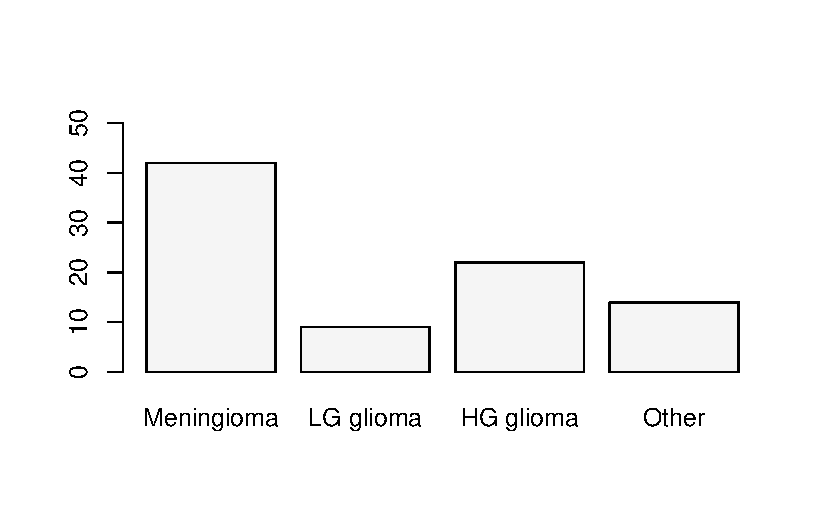
\includegraphics{./03-DescriptiveII_files/figure-pdf/unnamed-chunk-3-1.pdf}

}

\end{figure}

\begin{enumerate}
\def\labelenumi{\arabic{enumi}.}
\setcounter{enumi}{2}
\tightlist
\item
  \(33\) people did not survive Meningioma. The survival rate of
  Meningioma is only \(21.43\)\%.
\end{enumerate}

Use the \texttt{table()} function one more time to create the
contingency table for the two variables.

\begin{Shaded}
\begin{Highlighting}[numbers=left,,]
\NormalTok{(freq2}\OtherTok{\textless{}{-}}\FunctionTok{table}\NormalTok{(BrainCancer}\SpecialCharTok{$}\NormalTok{status,BrainCancer}\SpecialCharTok{$}\NormalTok{diagnosis))}
\end{Highlighting}
\end{Shaded}

\begin{verbatim}
   
    Meningioma LG glioma HG glioma Other
  0         33         5         5     9
  1          9         4        17     5
\end{verbatim}

To get the survival rates, we can use the \texttt{prop.table()} function
once again.

\begin{Shaded}
\begin{Highlighting}[numbers=left,,]
\FunctionTok{prop.table}\NormalTok{(freq2,}\AttributeTok{margin =} \DecValTok{2}\NormalTok{)}
\end{Highlighting}
\end{Shaded}

\begin{verbatim}
   
    Meningioma LG glioma HG glioma     Other
  0  0.7857143 0.5555556 0.2272727 0.6428571
  1  0.2142857 0.4444444 0.7727273 0.3571429
\end{verbatim}

\begin{enumerate}
\def\labelenumi{\arabic{enumi}.}
\setcounter{enumi}{3}
\tightlist
\item
  Meningioma and not surviving is the most common with \(33\)
  occurrences. High grade glioma and surviving is the the second most
  common.
\end{enumerate}

Use the \texttt{barplot()} function one more time to construct the
stacked column chart.

\begin{Shaded}
\begin{Highlighting}[numbers=left,,]
\FunctionTok{barplot}\NormalTok{(}\FunctionTok{table}\NormalTok{(BrainCancer}\SpecialCharTok{$}\NormalTok{status,BrainCancer}\SpecialCharTok{$}\NormalTok{diagnosis),}
        \AttributeTok{legend.text =} \FunctionTok{c}\NormalTok{(}\StringTok{"Not Survived"}\NormalTok{,}\StringTok{"Survived"}\NormalTok{), }\AttributeTok{ylim=}\FunctionTok{c}\NormalTok{(}\DecValTok{0}\NormalTok{,}\DecValTok{50}\NormalTok{))}
\end{Highlighting}
\end{Shaded}

\begin{figure}[H]

{\centering 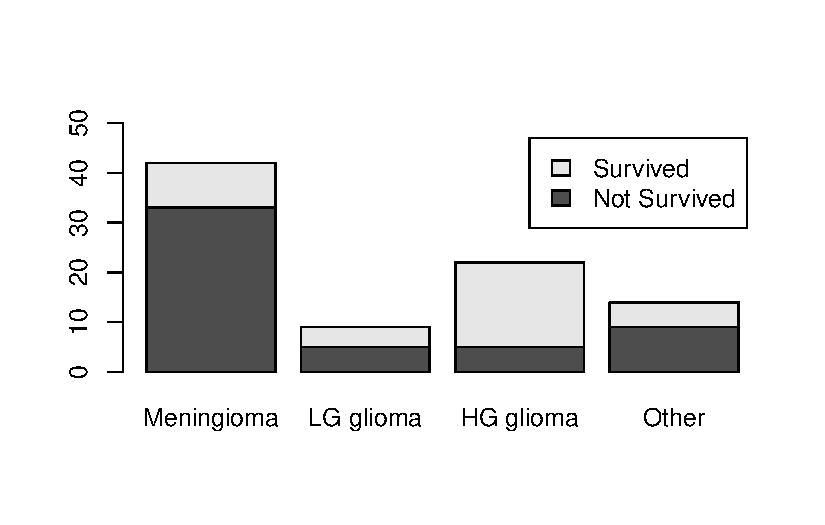
\includegraphics{./03-DescriptiveII_files/figure-pdf/unnamed-chunk-6-1.pdf}

}

\end{figure}

\hypertarget{exercise-2-3}{%
\subsection*{Exercise 2}\label{exercise-2-3}}
\addcontentsline{toc}{subsection}{Exercise 2}

\begin{enumerate}
\def\labelenumi{\arabic{enumi}.}
\tightlist
\item
  The highest frequency is in the \(80 < x ≤ 90\) bin. \(8\)
  temperatures were between \(50 < x ≤ 60\) degrees.
\end{enumerate}

Create a vector containing the intervals desired by using the
\texttt{seq()} function.

\begin{Shaded}
\begin{Highlighting}[numbers=left,,]
\NormalTok{intervals }\OtherTok{\textless{}{-}} \FunctionTok{seq}\NormalTok{(}\DecValTok{50}\NormalTok{, }\DecValTok{100}\NormalTok{, }\AttributeTok{by=}\DecValTok{10}\NormalTok{)}
\end{Highlighting}
\end{Shaded}

Next use the \texttt{cut()} function to create the cuts for the
histogram.

\begin{Shaded}
\begin{Highlighting}[numbers=left,,]
\NormalTok{intervals.cut }\OtherTok{\textless{}{-}} \FunctionTok{cut}\NormalTok{(airquality}\SpecialCharTok{$}\NormalTok{Temp, intervals, }\AttributeTok{left=}\ConstantTok{FALSE}\NormalTok{, }\AttributeTok{right=}\ConstantTok{TRUE}\NormalTok{)}
\end{Highlighting}
\end{Shaded}

The frequency distribution can be obtained by using the \texttt{table()}
function on the \emph{interval.cut} object created above.

\begin{Shaded}
\begin{Highlighting}[numbers=left,,]
\FunctionTok{table}\NormalTok{(intervals.cut)}
\end{Highlighting}
\end{Shaded}

\begin{verbatim}
intervals.cut
 (50,60]  (60,70]  (70,80]  (80,90] (90,100] 
       8       25       52       54       14 
\end{verbatim}

\begin{enumerate}
\def\labelenumi{\arabic{enumi}.}
\setcounter{enumi}{1}
\tightlist
\item
  The temperature was \(5.22\)\% of the time between \(50\) and \(60\);
  The temperature was \(70\) or less \(33\) times; The temperature was
  above \(70\), \(78.43\)\% of the time.
\end{enumerate}

To get the relative frequency table, start by saving the proportion
table into an object.Then you can use the \texttt{prop.table()}
function.

\begin{Shaded}
\begin{Highlighting}[numbers=left,,]
\NormalTok{freq}\OtherTok{\textless{}{-}}\FunctionTok{table}\NormalTok{(intervals.cut) }
\FunctionTok{prop.table}\NormalTok{(freq)}
\end{Highlighting}
\end{Shaded}

\begin{verbatim}
intervals.cut
   (50,60]    (60,70]    (70,80]    (80,90]   (90,100] 
0.05228758 0.16339869 0.33986928 0.35294118 0.09150327 
\end{verbatim}

For the cumulative distribution you can use the \texttt{cumsum()}
function on the frequency distribution.

\begin{Shaded}
\begin{Highlighting}[numbers=left,,]
\NormalTok{cumulfreq}\OtherTok{\textless{}{-}}\FunctionTok{cumsum}\NormalTok{(freq)}
\NormalTok{cumulfreq}
\end{Highlighting}
\end{Shaded}

\begin{verbatim}
 (50,60]  (60,70]  (70,80]  (80,90] (90,100] 
       8       33       85      139      153 
\end{verbatim}

Lastly, for the relative cumulative distribution table, you can use the
\texttt{cumsum()} function on the relative frequency table.

\begin{Shaded}
\begin{Highlighting}[numbers=left,,]
\FunctionTok{cumsum}\NormalTok{(}\FunctionTok{prop.table}\NormalTok{(freq))}
\end{Highlighting}
\end{Shaded}

\begin{verbatim}
   (50,60]    (60,70]    (70,80]    (80,90]   (90,100] 
0.05228758 0.21568627 0.55555556 0.90849673 1.00000000 
\end{verbatim}

\begin{enumerate}
\def\labelenumi{\arabic{enumi}.}
\setcounter{enumi}{2}
\tightlist
\item
  The distribution is not perfectly symmetric. It is skewed slightly to
  the left (see histogram.)
\end{enumerate}

Use the \texttt{hist()} function to create the histogram.

\begin{Shaded}
\begin{Highlighting}[numbers=left,,]
\FunctionTok{hist}\NormalTok{(airquality}\SpecialCharTok{$}\NormalTok{Temp, }\AttributeTok{breaks=}\NormalTok{intervals, }
     \AttributeTok{right=}\ConstantTok{TRUE}\NormalTok{,}\AttributeTok{col=}\StringTok{"\#F5F5F5"}\NormalTok{, }\AttributeTok{main=}\StringTok{"Temperature in NY"}\NormalTok{, }\AttributeTok{xlab=}\StringTok{""}\NormalTok{)}
\end{Highlighting}
\end{Shaded}

\begin{figure}[H]

{\centering 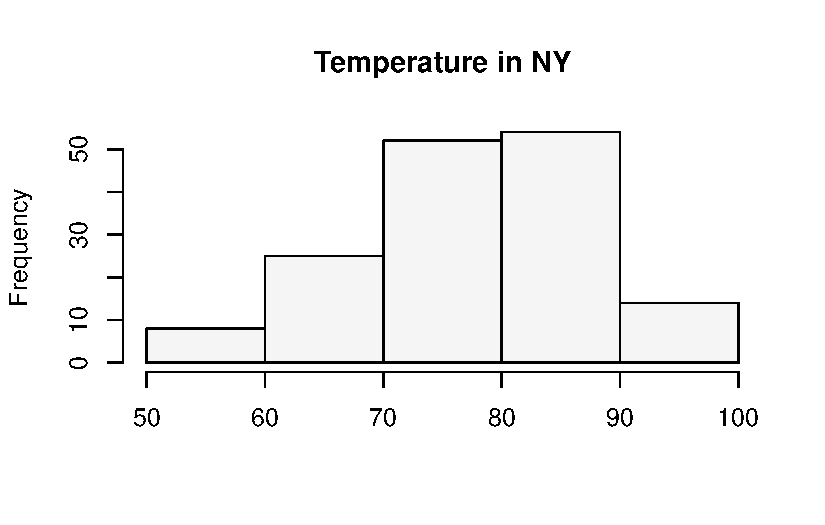
\includegraphics{./03-DescriptiveII_files/figure-pdf/unnamed-chunk-13-1.pdf}

}

\end{figure}

\hypertarget{exercise-3-3}{%
\subsection*{Exercise 3}\label{exercise-3-3}}
\addcontentsline{toc}{subsection}{Exercise 3}

\begin{enumerate}
\def\labelenumi{\arabic{enumi}.}
\tightlist
\item
  From \(1901\) through \(2000\), both portfolios have behaved very
  similarly. Returns are between \(-3\)\% and \(3\)\%, there is no
  trend, and positive (negative) returns for X seem to match with
  positive (negative) returns of Y.
\end{enumerate}

You can use the \texttt{plot()} function to create a plot of Portfolio
Y. The line for Portfolio X can be added with the \texttt{lines()}
function.

\begin{Shaded}
\begin{Highlighting}[numbers=left,,]
\FunctionTok{plot}\NormalTok{(Portfolio}\SpecialCharTok{$}\NormalTok{Y, }
     \AttributeTok{x=}\FunctionTok{seq}\NormalTok{(}\DecValTok{1901}\NormalTok{,}\DecValTok{2000}\NormalTok{), }\AttributeTok{type=}\StringTok{"l"}\NormalTok{, }
     \AttributeTok{col=}\StringTok{"black"}\NormalTok{, }\AttributeTok{xlab=}\StringTok{""}\NormalTok{, }\AttributeTok{ylab=}\StringTok{"\% Return"}\NormalTok{, }\AttributeTok{ylim=}\FunctionTok{c}\NormalTok{(}\SpecialCharTok{{-}}\DecValTok{3}\NormalTok{,}\DecValTok{3}\NormalTok{), }
     \AttributeTok{xlim=}\FunctionTok{c}\NormalTok{(}\DecValTok{1901}\NormalTok{,}\DecValTok{2000}\NormalTok{), }\AttributeTok{lwd=}\DecValTok{2}\NormalTok{, }\AttributeTok{axes =}\NormalTok{ F)}
\FunctionTok{axis}\NormalTok{(}\AttributeTok{side=}\DecValTok{1}\NormalTok{, }\AttributeTok{labels=}\ConstantTok{TRUE}\NormalTok{, }\AttributeTok{font=}\DecValTok{1}\NormalTok{,}\AttributeTok{las=}\DecValTok{1}\NormalTok{)}
\FunctionTok{axis}\NormalTok{(}\AttributeTok{side=}\DecValTok{2}\NormalTok{, }\AttributeTok{labels=}\ConstantTok{TRUE}\NormalTok{, }\AttributeTok{font=}\DecValTok{1}\NormalTok{,}\AttributeTok{las=}\DecValTok{1}\NormalTok{)}
\FunctionTok{lines}\NormalTok{(Portfolio}\SpecialCharTok{$}\NormalTok{X, }\AttributeTok{x=}\FunctionTok{seq}\NormalTok{(}\DecValTok{1901}\NormalTok{,}\DecValTok{2000}\NormalTok{), }\AttributeTok{type=}\StringTok{"l"}\NormalTok{, }
      \AttributeTok{col=}\StringTok{"darkgrey"}\NormalTok{, }\AttributeTok{lwd=}\DecValTok{2}\NormalTok{)}
\FunctionTok{legend}\NormalTok{(}\AttributeTok{x =} \StringTok{"bottomleft"}\NormalTok{,          }
       \AttributeTok{legend =} \FunctionTok{c}\NormalTok{(}\StringTok{"Port Y"}\NormalTok{, }\StringTok{"Port X"}\NormalTok{),  }
       \AttributeTok{lty =} \FunctionTok{c}\NormalTok{(}\DecValTok{1}\NormalTok{, }\DecValTok{1}\NormalTok{),           }
       \AttributeTok{col =} \FunctionTok{c}\NormalTok{(}\StringTok{"black"}\NormalTok{, }\StringTok{"darkgrey"}\NormalTok{),         }
       \AttributeTok{lwd =} \DecValTok{2}\NormalTok{,}
       \AttributeTok{bty=}\StringTok{"n"}\NormalTok{)                }
\end{Highlighting}
\end{Shaded}

\begin{figure}[H]

{\centering 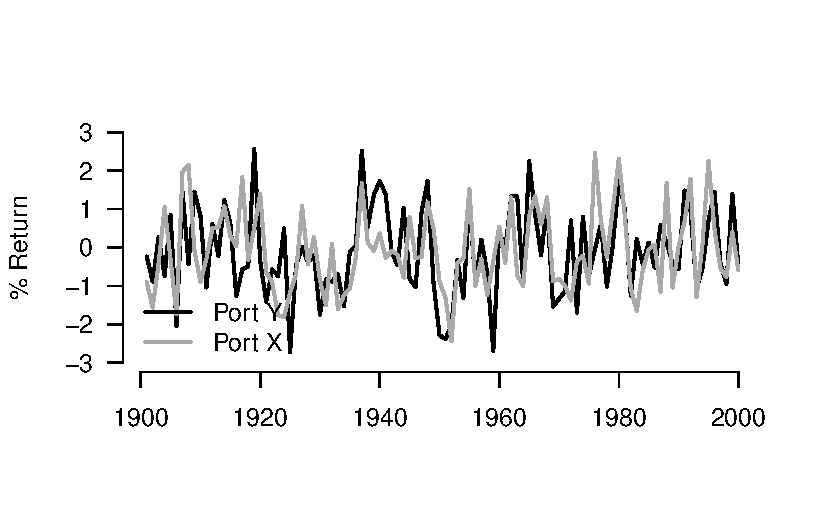
\includegraphics{./03-DescriptiveII_files/figure-pdf/unnamed-chunk-14-1.pdf}

}

\end{figure}

\hypertarget{descriptive-statistics-iii}{%
\chapter{Descriptive Statistics III}\label{descriptive-statistics-iii}}

\hypertarget{concepts-2}{%
\section{Concepts}\label{concepts-2}}

\hypertarget{measures-of-central-location}{%
\subsection*{Measures of Central
Location}\label{measures-of-central-location}}
\addcontentsline{toc}{subsection}{Measures of Central Location}

Measures of Central Location determine where the center of a
distribution lies.

\begin{itemize}
\item
  The \textbf{mean} is the average value for a numerical variable. The
  sample statistic is estimated by \(\bar{x}=\sum x_{i}/n\), where
  \(x_i\) is observation \(i\), and \(n\) is the number of observations.
  The population parameter is defined as \(\mu=\sum x_{i}/N\).
\item
  The \textbf{median} is the value in the middle when data is organized
  in ascending order. When \(n\) is even, the median is the average
  between the two middle values.
\item
  The \textbf{mode} is the value with highest frequency from a set of
  observations.
\item
  The \textbf{weighted mean} uses weights to determine the importance of
  each data point of a variable. It is calculated by
  \(\frac{\sum w_{i}x_{i}}{\sum w_{i}}\), where \(w_{i}\) are the
  weights associated to the values \(x_{i}\).
\item
  The \textbf{geometric mean} is a multiplicative average that is less
  sensitive to outliers. It is used to average growth rates or rated of
  return. It is calculated by \(\sqrt[n]{(1+r_1)*(1+r_2)...(1+r_n)}-1\),
  where \(\sqrt[n]{}\) is the \(n_{th}\) root, and \(r_i\) are the
  returns or growth rates.
\end{itemize}

\hypertarget{useful-r-functions-2}{%
\subsection*{Useful R functions}\label{useful-r-functions-2}}
\addcontentsline{toc}{subsection}{Useful R functions}

Base R has a collection of functions that calculate measures of central
location.

\begin{itemize}
\item
  The \texttt{mean()} function calculates the average of a vector of
  values.
\item
  The \texttt{median()} function returns the median of a vector of
  values.
\item
  The \texttt{table()} function provides us with a frequency
  distribution. We can then identify the mode(s) of the vector provided.
\item
  The \texttt{summary()} function returns a collection of descriptive
  statistics for a vector or data frame.
\end{itemize}

\hypertarget{exercises-2}{%
\section{Exercises}\label{exercises-2}}

The following exercises will help you practice the measures of central
location. In particular, the exercises work on:

\begin{itemize}
\item
  Calculating the mean, median, and the mode.
\item
  Calculating the weighted average.
\item
  Applying the geometric mean for growth rates and returns.
\end{itemize}

Answers are provided below. Try not to peak until you have a formulated
your own answer and double checked your work for any mistakes.

\hypertarget{exercise-1-4}{%
\subsection*{Exercise 1}\label{exercise-1-4}}
\addcontentsline{toc}{subsection}{Exercise 1}

For the following exercises, make your calculations by hand and verify
results using R functions when possible.

\begin{enumerate}
\def\labelenumi{\arabic{enumi}.}
\item
  Use the following observations to calculate the mean, the median, and
  the mode.

  \begin{longtable}[]{@{}ccccc@{}}
  \toprule()
  \endhead
  8 & 10 & 9 & 12 & 12 \\
  \bottomrule()
  \end{longtable}
\item
  Use following observations to calculate the mean, the median, and the
  mode.

  \begin{longtable}[]{@{}cccccc@{}}
  \toprule()
  \endhead
  -4 & 0 & -6 & 1 & -3 & -4 \\
  \bottomrule()
  \end{longtable}
\item
  Use the following observations, calculate the mean, the median, and
  the mode.

  \begin{longtable}[]{@{}ccccccccc@{}}
  \toprule()
  \endhead
  20 & 15 & 25 & 20 & 10 & 15 & 25 & 20 & 15 \\
  \bottomrule()
  \end{longtable}
\end{enumerate}

\hypertarget{exercise-2-4}{%
\subsection*{Exercise 2}\label{exercise-2-4}}
\addcontentsline{toc}{subsection}{Exercise 2}

Download the \texttt{ISLR2} package. You will need the \textbf{OJ} data
set to answer this question.

\begin{enumerate}
\def\labelenumi{\arabic{enumi}.}
\item
  Find the mean price for Country Hill (\emph{PriceCH}) and Minute Maid
  (\emph{PriceMM}).
\item
  Find the mean price of Country Hill (\emph{PriceCH}) in store 1 and
  store 2 (\emph{StoreID}). Which store had the better price?
\item
  Find the mean price paid by Country Hill (\emph{PriceCH}) purchasers
  (\emph{Purchase}) in store 1 (\emph{StoreID})? How about store 2?
  Which store had the better price?
\end{enumerate}

\hypertarget{exercise-3-4}{%
\subsection*{Exercise 3}\label{exercise-3-4}}
\addcontentsline{toc}{subsection}{Exercise 3}

\begin{enumerate}
\def\labelenumi{\arabic{enumi}.}
\tightlist
\item
  Over the past year an investor bought TSLA. She made these purchases
  on three occasions at the prices shown in the table below. Calculate
  the average price per share.
\end{enumerate}

\begin{longtable}[]{@{}ccc@{}}
\toprule()
Date & Price Per Share & Number of Shares \\
\midrule()
\endhead
February & 250.34 & 80 \\
April & 234.59 & 120 \\
Aug & 270.45 & 50 \\
\bottomrule()
\end{longtable}

\begin{enumerate}
\def\labelenumi{\arabic{enumi}.}
\setcounter{enumi}{1}
\tightlist
\item
  What would have been the average price per share if the investor would
  have bought equal amounts of shares each month?
\end{enumerate}

\hypertarget{exercise-4}{%
\subsection*{Exercise 4}\label{exercise-4}}
\addcontentsline{toc}{subsection}{Exercise 4}

\begin{enumerate}
\def\labelenumi{\arabic{enumi}.}
\item
  Consider the following observations for the consumer price index
  (CPI). Calculate the inflation rate (Growth Rate of the CPI) for each
  period.

  \begin{longtable}[]{@{}ccccc@{}}
  \toprule()
  \endhead
  1.0 & 1.3 & 1.6 & 1.8 & 2.1 \\
  \bottomrule()
  \end{longtable}
\item
  Suppose that you want to invest \$1000 dollars in a stock that is
  predicted to yield the following returns in the next four years.
  Calculate both the arithmetic mean and the geometric mean. Use the
  geometric mean to estimate how much money you would have by the end of
  year 4.

  \begin{longtable}[]{@{}cc@{}}
  \toprule()
  Year & Annual Return \\
  \midrule()
  \endhead
  1 & 17.3 \\
  2 & 19.6 \\
  3 & 6.8 \\
  4 & 8.2 \\
  \bottomrule()
  \end{longtable}
\end{enumerate}

\hypertarget{answers-2}{%
\section{Answers}\label{answers-2}}

\hypertarget{exercise-1-5}{%
\subsection*{Exercise 1}\label{exercise-1-5}}
\addcontentsline{toc}{subsection}{Exercise 1}

\begin{enumerate}
\def\labelenumi{\arabic{enumi}.}
\item
  To find the mean we will use the following formula
  \(( \frac{1}{n} \sum_{i=i}^{n} x_{i})\). The summation of the values
  is \(51\) and the number of observations is \(5\). The mean is
  \(51/5=10.2\).

  The median is found by locating the middle value when data is sorted
  in ascending order. The median in this example is \(10\).

  The mode is the value with the highest frequency. In this example the
  mode is \(12\) since it is repeated twice and all other numbers appear
  only once.
\end{enumerate}

The mean can be easily verified in R by using the \texttt{mean()}
function:

\begin{Shaded}
\begin{Highlighting}[numbers=left,,]
\FunctionTok{mean}\NormalTok{(}\FunctionTok{c}\NormalTok{(}\DecValTok{8}\NormalTok{,}\DecValTok{10}\NormalTok{,}\DecValTok{9}\NormalTok{,}\DecValTok{12}\NormalTok{,}\DecValTok{12}\NormalTok{))}
\end{Highlighting}
\end{Shaded}

\begin{verbatim}
[1] 10.2
\end{verbatim}

Similarly, the median is easily verified by using the \texttt{median()}
function:

\begin{Shaded}
\begin{Highlighting}[numbers=left,,]
\FunctionTok{median}\NormalTok{(}\FunctionTok{c}\NormalTok{(}\DecValTok{8}\NormalTok{,}\DecValTok{10}\NormalTok{,}\DecValTok{9}\NormalTok{,}\DecValTok{12}\NormalTok{,}\DecValTok{12}\NormalTok{))}
\end{Highlighting}
\end{Shaded}

\begin{verbatim}
[1] 10
\end{verbatim}

We can use the \texttt{table()} function to calculate frequencies and
easily identify the mode.

\begin{Shaded}
\begin{Highlighting}[numbers=left,,]
\FunctionTok{table}\NormalTok{(}\FunctionTok{c}\NormalTok{(}\DecValTok{8}\NormalTok{,}\DecValTok{10}\NormalTok{,}\DecValTok{9}\NormalTok{,}\DecValTok{12}\NormalTok{,}\DecValTok{12}\NormalTok{))}
\end{Highlighting}
\end{Shaded}

\begin{verbatim}

 8  9 10 12 
 1  1  1  2 
\end{verbatim}

\begin{enumerate}
\def\labelenumi{\arabic{enumi}.}
\setcounter{enumi}{1}
\tightlist
\item
  The mean is \(-2.67\), the median is \(-3.5\), the mode is \(-4\).
\end{enumerate}

These mean is verified in R:

\begin{Shaded}
\begin{Highlighting}[numbers=left,,]
\FunctionTok{mean}\NormalTok{(}\FunctionTok{c}\NormalTok{(}\SpecialCharTok{{-}}\DecValTok{4}\NormalTok{,}\DecValTok{0}\NormalTok{,}\SpecialCharTok{{-}}\DecValTok{6}\NormalTok{,}\DecValTok{1}\NormalTok{,}\SpecialCharTok{{-}}\DecValTok{3}\NormalTok{,}\SpecialCharTok{{-}}\DecValTok{4}\NormalTok{))}
\end{Highlighting}
\end{Shaded}

\begin{verbatim}
[1] -2.666667
\end{verbatim}

The median in R:

\begin{Shaded}
\begin{Highlighting}[numbers=left,,]
\FunctionTok{median}\NormalTok{(}\FunctionTok{c}\NormalTok{(}\SpecialCharTok{{-}}\DecValTok{4}\NormalTok{,}\DecValTok{0}\NormalTok{,}\SpecialCharTok{{-}}\DecValTok{6}\NormalTok{,}\DecValTok{1}\NormalTok{,}\SpecialCharTok{{-}}\DecValTok{3}\NormalTok{,}\SpecialCharTok{{-}}\DecValTok{4}\NormalTok{))}
\end{Highlighting}
\end{Shaded}

\begin{verbatim}
[1] -3.5
\end{verbatim}

Finally, the mode in R:

\begin{Shaded}
\begin{Highlighting}[numbers=left,,]
\FunctionTok{table}\NormalTok{(}\FunctionTok{c}\NormalTok{(}\SpecialCharTok{{-}}\DecValTok{4}\NormalTok{,}\DecValTok{0}\NormalTok{,}\SpecialCharTok{{-}}\DecValTok{6}\NormalTok{,}\DecValTok{1}\NormalTok{,}\SpecialCharTok{{-}}\DecValTok{3}\NormalTok{,}\SpecialCharTok{{-}}\DecValTok{4}\NormalTok{))}
\end{Highlighting}
\end{Shaded}

\begin{verbatim}

-6 -4 -3  0  1 
 1  2  1  1  1 
\end{verbatim}

\begin{enumerate}
\def\labelenumi{\arabic{enumi}.}
\setcounter{enumi}{2}
\tightlist
\item
  The mean is \(18.33\), the median is \(20\), the data is bimodal with
  both \(15\) and \(20\) being modes.
\end{enumerate}

These mean is verified in R:

\begin{Shaded}
\begin{Highlighting}[numbers=left,,]
\FunctionTok{mean}\NormalTok{(}\FunctionTok{c}\NormalTok{(}\DecValTok{20}\NormalTok{,}\DecValTok{15}\NormalTok{,}\DecValTok{25}\NormalTok{,}\DecValTok{20}\NormalTok{,}\DecValTok{10}\NormalTok{,}\DecValTok{15}\NormalTok{,}\DecValTok{25}\NormalTok{,}\DecValTok{20}\NormalTok{,}\DecValTok{15}\NormalTok{))}
\end{Highlighting}
\end{Shaded}

\begin{verbatim}
[1] 18.33333
\end{verbatim}

The median in R:

\begin{Shaded}
\begin{Highlighting}[numbers=left,,]
\FunctionTok{median}\NormalTok{(}\FunctionTok{c}\NormalTok{(}\DecValTok{20}\NormalTok{,}\DecValTok{15}\NormalTok{,}\DecValTok{25}\NormalTok{,}\DecValTok{20}\NormalTok{,}\DecValTok{10}\NormalTok{,}\DecValTok{15}\NormalTok{,}\DecValTok{25}\NormalTok{,}\DecValTok{20}\NormalTok{,}\DecValTok{15}\NormalTok{))}
\end{Highlighting}
\end{Shaded}

\begin{verbatim}
[1] 20
\end{verbatim}

The frequency distribution identifies the modes:

\begin{Shaded}
\begin{Highlighting}[numbers=left,,]
\FunctionTok{table}\NormalTok{(}\FunctionTok{c}\NormalTok{(}\DecValTok{20}\NormalTok{,}\DecValTok{15}\NormalTok{,}\DecValTok{25}\NormalTok{,}\DecValTok{20}\NormalTok{,}\DecValTok{10}\NormalTok{,}\DecValTok{15}\NormalTok{,}\DecValTok{25}\NormalTok{,}\DecValTok{20}\NormalTok{,}\DecValTok{15}\NormalTok{))}
\end{Highlighting}
\end{Shaded}

\begin{verbatim}

10 15 20 25 
 1  3  3  2 
\end{verbatim}

\hypertarget{exercise-2-5}{%
\subsection*{Exercise 2}\label{exercise-2-5}}
\addcontentsline{toc}{subsection}{Exercise 2}

\begin{enumerate}
\def\labelenumi{\arabic{enumi}.}
\tightlist
\item
  The mean price for Country Hill is \(1.87\). The mean price for Minute
  Maid is \(2.09\).
\end{enumerate}

The means can be easily found with the \texttt{mean()} function:

\begin{Shaded}
\begin{Highlighting}[numbers=left,,]
\FunctionTok{library}\NormalTok{(ISLR2)}
\FunctionTok{mean}\NormalTok{(OJ}\SpecialCharTok{$}\NormalTok{PriceCH)}
\end{Highlighting}
\end{Shaded}

\begin{verbatim}
[1] 1.867421
\end{verbatim}

\begin{Shaded}
\begin{Highlighting}[numbers=left,,]
\FunctionTok{mean}\NormalTok{(OJ}\SpecialCharTok{$}\NormalTok{PriceMM)}
\end{Highlighting}
\end{Shaded}

\begin{verbatim}
[1] 2.085411
\end{verbatim}

\begin{enumerate}
\def\labelenumi{\arabic{enumi}.}
\setcounter{enumi}{1}
\tightlist
\item
  The mean price at store 1 for Country Hill is \(1.80\) vs.~\(1.84\)
  for store 2. The juice is cheaper at store 1.
\end{enumerate}

The means for each store can be found by using indexing and a logical
statement. The Country Hill mean price at store 1 is given by:

\begin{Shaded}
\begin{Highlighting}[numbers=left,,]
\FunctionTok{mean}\NormalTok{(OJ}\SpecialCharTok{$}\NormalTok{PriceCH[OJ}\SpecialCharTok{$}\NormalTok{StoreID}\SpecialCharTok{==}\DecValTok{1}\NormalTok{])}
\end{Highlighting}
\end{Shaded}

\begin{verbatim}
[1] 1.803758
\end{verbatim}

The Country Hill mean price at store 2 is given by:

\begin{Shaded}
\begin{Highlighting}[numbers=left,,]
\FunctionTok{mean}\NormalTok{(OJ}\SpecialCharTok{$}\NormalTok{PriceCH[OJ}\SpecialCharTok{$}\NormalTok{StoreID}\SpecialCharTok{==}\DecValTok{2}\NormalTok{])}
\end{Highlighting}
\end{Shaded}

\begin{verbatim}
[1] 1.841216
\end{verbatim}

\begin{enumerate}
\def\labelenumi{\arabic{enumi}.}
\setcounter{enumi}{2}
\tightlist
\item
  Purchasers of Country Hill at store 1 paid and average of \(1.80\) for
  Country Hill juice. At store 2 they paid \(1.86\). Once again the
  average price was lower at store 1.
\end{enumerate}

The mean for Country Hill purchasers at store 1 is given by:

\begin{Shaded}
\begin{Highlighting}[numbers=left,,]
\FunctionTok{mean}\NormalTok{(OJ}\SpecialCharTok{$}\NormalTok{PriceCH[OJ}\SpecialCharTok{$}\NormalTok{StoreID}\SpecialCharTok{==}\DecValTok{1} \SpecialCharTok{\&}\NormalTok{ OJ}\SpecialCharTok{$}\NormalTok{Purchase}\SpecialCharTok{==}\StringTok{"CH"}\NormalTok{])}
\end{Highlighting}
\end{Shaded}

\begin{verbatim}
[1] 1.797176
\end{verbatim}

The mean for Country Hill purchasers at store 2 is:

\begin{Shaded}
\begin{Highlighting}[numbers=left,,]
\FunctionTok{mean}\NormalTok{(OJ}\SpecialCharTok{$}\NormalTok{PriceCH[OJ}\SpecialCharTok{$}\NormalTok{StoreID}\SpecialCharTok{==}\DecValTok{2} \SpecialCharTok{\&}\NormalTok{ OJ}\SpecialCharTok{$}\NormalTok{Purchase}\SpecialCharTok{==}\StringTok{"CH"}\NormalTok{])}
\end{Highlighting}
\end{Shaded}

\begin{verbatim}
[1] 1.857383
\end{verbatim}

\hypertarget{exercise-3-5}{%
\subsection*{Exercise 3}\label{exercise-3-5}}
\addcontentsline{toc}{subsection}{Exercise 3}

\begin{enumerate}
\def\labelenumi{\arabic{enumi}.}
\tightlist
\item
  The average price of sale is found by using the weighted average
  formula. \(\frac{\sum w_{i}x_{i}}{\sum w_{i}}\) The weights
  (\(w_{i}\)) are given by the number of shares bought and the values
  (\(x_{i}\)) are the prices. The weighted average is \(246.802\).
\end{enumerate}

In R you can create two vectors. One holds the share price and the other
one the number of shares bought.

\begin{Shaded}
\begin{Highlighting}[numbers=left,,]
\NormalTok{PricePerShare}\OtherTok{\textless{}{-}}\FunctionTok{c}\NormalTok{(}\FloatTok{250.34}\NormalTok{,}\FloatTok{234.59}\NormalTok{,}\FloatTok{270.45}\NormalTok{)}
\NormalTok{NumberOfShares}\OtherTok{\textless{}{-}}\FunctionTok{c}\NormalTok{(}\DecValTok{80}\NormalTok{,}\DecValTok{120}\NormalTok{,}\DecValTok{50}\NormalTok{)}
\end{Highlighting}
\end{Shaded}

Next, you can multiply the \emph{PricePerShare} and
\emph{NumberOfShares} vectors to find the numerator and then use
\texttt{sum()} function to find the denominator. The weighted average
is:

\begin{Shaded}
\begin{Highlighting}[numbers=left,,]
\NormalTok{(WeightedAverage}\OtherTok{\textless{}{-}}
  \FunctionTok{sum}\NormalTok{(PricePerShare}\SpecialCharTok{*}\NormalTok{NumberOfShares)}\SpecialCharTok{/}\FunctionTok{sum}\NormalTok{(NumberOfShares))}
\end{Highlighting}
\end{Shaded}

\begin{verbatim}
[1] 246.802
\end{verbatim}

\begin{enumerate}
\def\labelenumi{\arabic{enumi}.}
\setcounter{enumi}{1}
\tightlist
\item
  The average if equal shares were bought would be \(251.7933\).
\end{enumerate}

In R you can use the \texttt{mean()} function on the PricePerShare
vector.

\begin{Shaded}
\begin{Highlighting}[numbers=left,,]
\NormalTok{(Average}\OtherTok{\textless{}{-}}\FunctionTok{mean}\NormalTok{(PricePerShare))}
\end{Highlighting}
\end{Shaded}

\begin{verbatim}
[1] 251.7933
\end{verbatim}

\hypertarget{exercise-4-1}{%
\subsection*{Exercise 4}\label{exercise-4-1}}
\addcontentsline{toc}{subsection}{Exercise 4}

\begin{enumerate}
\def\labelenumi{\arabic{enumi}.}
\tightlist
\item
  The inflation rate for each period is shown in the table below:
\end{enumerate}

\begin{longtable}[]{@{}cccc@{}}
\toprule()
\endhead
30\% & 23.08\% & 12.5\% & 16.67\% \\
\bottomrule()
\end{longtable}

In R create an object to store the values of the CPI:

\begin{Shaded}
\begin{Highlighting}[numbers=left,,]
\NormalTok{CPI}\OtherTok{\textless{}{-}}\FunctionTok{c}\NormalTok{(}\DecValTok{1}\NormalTok{,}\FloatTok{1.3}\NormalTok{,}\FloatTok{1.6}\NormalTok{,}\FloatTok{1.8}\NormalTok{,}\FloatTok{2.1}\NormalTok{)}
\end{Highlighting}
\end{Shaded}

Next use the \texttt{diff()} function to find the difference between the
end value and start value. Divide the result by a vector of starting
value and multiply times 100.

\begin{Shaded}
\begin{Highlighting}[numbers=left,,]
\NormalTok{(Inflation}\OtherTok{\textless{}{-}}\DecValTok{100}\SpecialCharTok{*}\FunctionTok{diff}\NormalTok{(CPI)}\SpecialCharTok{/}\NormalTok{CPI[}\DecValTok{1}\SpecialCharTok{:}\DecValTok{4}\NormalTok{])}
\end{Highlighting}
\end{Shaded}

\begin{verbatim}
[1] 30.00000 23.07692 12.50000 16.66667
\end{verbatim}

\begin{enumerate}
\def\labelenumi{\arabic{enumi}.}
\setcounter{enumi}{1}
\tightlist
\item
  At the end of 4 years it is predicted that you would have \(1621.17\)
  dollars. Each year you would have gained \(12.84\)\% on average.
\end{enumerate}

In R include the annual rates in a vector:

\begin{Shaded}
\begin{Highlighting}[numbers=left,,]
\NormalTok{growth}\OtherTok{\textless{}{-}}\FunctionTok{c}\NormalTok{(}\FloatTok{0.173}\NormalTok{,}\FloatTok{0.196}\NormalTok{,}\FloatTok{0.068}\NormalTok{,}\FloatTok{0.082}\NormalTok{)}
\end{Highlighting}
\end{Shaded}

The arithmetic mean is:

\begin{Shaded}
\begin{Highlighting}[numbers=left,,]
\DecValTok{100}\SpecialCharTok{*}\FunctionTok{mean}\NormalTok{(growth)}
\end{Highlighting}
\end{Shaded}

\begin{verbatim}
[1] 12.975
\end{verbatim}

The geometric mean is:

\begin{Shaded}
\begin{Highlighting}[numbers=left,,]
\NormalTok{(geom}\OtherTok{\textless{}{-}}\NormalTok{((}\FunctionTok{prod}\NormalTok{(}\DecValTok{1}\SpecialCharTok{+}\NormalTok{growth))}\SpecialCharTok{\^{}}\NormalTok{(}\DecValTok{1}\SpecialCharTok{/}\DecValTok{4}\NormalTok{)}\SpecialCharTok{{-}}\DecValTok{1}\NormalTok{)}\SpecialCharTok{*}\DecValTok{100}\NormalTok{)}
\end{Highlighting}
\end{Shaded}

\begin{verbatim}
[1] 12.8384
\end{verbatim}

At the end of the four years we would have:

\begin{Shaded}
\begin{Highlighting}[numbers=left,,]
\DecValTok{1000}\SpecialCharTok{*}\NormalTok{(}\DecValTok{1}\SpecialCharTok{+}\NormalTok{geom}\SpecialCharTok{/}\DecValTok{100}\NormalTok{)}\SpecialCharTok{\^{}}\DecValTok{4}
\end{Highlighting}
\end{Shaded}

\begin{verbatim}
[1] 1621.167
\end{verbatim}

\bookmarksetup{startatroot}

\hypertarget{references}{%
\chapter*{References}\label{references}}
\addcontentsline{toc}{chapter}{References}

\markboth{References}{References}

\hypertarget{refs}{}
\begin{CSLReferences}{1}{0}
\leavevmode\vadjust pre{\hypertarget{ref-HOP}{}}%
Grolemund, Garret. 2014. {``Hands-on Programming with r.''}
\url{https://jjallaire.github.io/hopr/}.

\leavevmode\vadjust pre{\hypertarget{ref-R4DS}{}}%
Wickham, Hadley. 2017. {``R for Data Science.''}
\url{https://r4ds.hadley.nz}.

\end{CSLReferences}



\printindex

\end{document}
